\documentclass[12pt,a4paper]{iopart}

% Document information
\newcommand{\DRN}{GridPP-ENG-002-UserGuide}
\newcommand{\thisversion}{1.0}

% Author information
% Author information for T. Whyntie
\newcommand{\theauthorinit}{T Whyntie}
\newcommand{\theauthorfull}{Tom Whyntie}

\newcommand{\theauthoraddressA}{%
Particle Physics Research Centre, %
School of Physics and Astronomy, %
Queen Mary University of London, %
Mile End Road, London, E1 4NS, United Kingdom}
%
\newcommand{\theauthoremail}{t.whyntie@qmul.ac.uk}


% Packages and settings for GridPP document formatting
% Packages and settings for GridPP document formatting.

% Graphics
\usepackage[xetex]{graphicx}
\usepackage{subcaption}
\usepackage{enumerate}

% Tables
\usepackage{array}
\usepackage{dcolumn}
\newcolumntype{.}{D{.}{.}{2}}
\newcolumntype{C}[1]{>{\centering\let\newline\\\arraybackslash\hspace{0pt}}m{#1}}
% For the width of the "Services" column.
\newcommand*{\servw}{1.0cm}

% Layout
\usepackage{layouts}
\usepackage{lscape}
\usepackage{parskip}

% Sections
\usepackage[titletoc]{appendix}

% Colours
\usepackage{xcolor}
\definecolor{black}{RGB}{0,0,0}
\definecolor{grey}{RGB}{0.5,0.5,0.5}
\definecolor{gridppdarkblue}{RGB}{11,45,131}
\definecolor{gridpplightblue}{RGB}{133,150,193}
\definecolor{cernblue}{RGB}{0,85,160}

% Mathematics
\usepackage{latexsym}

% Fonts
\usepackage{fontspec,xunicode}
\defaultfontfeatures{Mapping=tex-text,Scale=MatchLowercase}
\setmainfont{Latin Modern Sans}

% Headers and footers
%
% Using the fancyhdr package for the, um, fancy headings...
\usepackage{fancyhdr}
\setlength{\headheight}{16pt}
\setlength{\voffset}{-0.3in}
\pagestyle{fancy}
%
% Redefine the IOP article header settings for the first page.
\makeatletter
\def\ps@myheadings{%
%    \let\@oddfoot\@empty\let\@evenfoot\@empty
    \let\@oddhead\@empty\let\@evenhead\@empty
    \let\@mkboth\@gobbletwo
    \let\sectionmark\@gobble
    \let\subsectionmark\@gobble}
\makeatother
\lhead{\sffamily\rightmark}
\rhead{\sffamily\leftmark}
\lfoot{\sffamily{\DRN-v\thisversion}}
\cfoot{}
\rfoot{\sffamily{\thepage}}

% Exercises/questions
\usepackage[listings]{tcolorbox}
\tcbset{before={\par\medskip\pagebreak[0]\noindent},after={\par\medskip}}%

% Warning tcolorbox
% #1: tcolorbox options
% #2: Box title
\newtcolorbox{warningbox}[2][]
{
  colframe = red!25,
  colback  = red!10,
  coltitle = red!20!black,  
  title    = #2,
  #1,
}

% Hint tcolorbox
% #1: tcolorbox options
% #2: Box title
\newtcolorbox{hintbox}[2][]
{
  colframe = green!25,
  colback  = green!10,
  coltitle = green!20!black,  
  title    = #2,
  #1,
}

% Info (information) tcolorbox
% #1: tcolorbox options
% #2: Box title
\newtcolorbox{infobox}[2][]
{
  colframe = grey!25,
  colback  = grey!10,
  coltitle = grey!20!black,  
  title    = #2,
  #1,
}

% Coding
\usepackage{listings}
% Listing options
\definecolor{listbacking}{rgb}{0.98,0.98,0.98}
\definecolor{commentgrey}{rgb}{0.60,0.60,0.60}
\definecolor{keywordblue}{rgb}{0.00,0.00,0.50}
\definecolor{stringgreen}{rgb}{0.00,0.50,0.00}
\definecolor{deepred}{rgb}{0.60,0.00,0.00}
\lstset{
  basicstyle=\footnotesize\ttfamily,
  gobble=4,
  float=hbtp,
  emph={__init__},
  emphstyle=\color{deepred},
  showspaces=false,
  showstringspaces=false,
  backgroundcolor=\color{listbacking},
  commentstyle=\color{commentgrey},
  stringstyle=\color{stringgreen},
  keywordstyle=\color{keywordblue},
  numbers=left,
  numbersep=12pt,
  %framexleftmargin=20pt,
  %framexrightmargin=20pt,
  stepnumber=1,
  showlines=true
}

% Pandoc coding.
\usepackage{fancyvrb}
\newcommand{\VerbBar}{|}
\newcommand{\VERB}{\Verb[commandchars=\\\{\}]}
\DefineVerbatimEnvironment{Highlighting}{Verbatim}{commandchars=\\\{\},fontsize=\small}
\newenvironment{Shaded}{}{}
\newcommand{\KeywordTok}[1]{\textcolor[rgb]{0.00,0.44,0.13}{\textbf{{#1}}}}
\newcommand{\DataTypeTok}[1]{\textcolor[rgb]{0.56,0.13,0.00}{{#1}}}
\newcommand{\DecValTok}[1]{\textcolor[rgb]{0.25,0.63,0.44}{{#1}}}
\newcommand{\BaseNTok}[1]{\textcolor[rgb]{0.25,0.63,0.44}{{#1}}}
\newcommand{\FloatTok}[1]{\textcolor[rgb]{0.25,0.63,0.44}{{#1}}}
\newcommand{\ConstantTok}[1]{\textcolor[rgb]{0.53,0.00,0.00}{{#1}}}
\newcommand{\CharTok}[1]{\textcolor[rgb]{0.25,0.44,0.63}{{#1}}}
\newcommand{\SpecialCharTok}[1]{\textcolor[rgb]{0.25,0.44,0.63}{{#1}}}
\newcommand{\StringTok}[1]{\textcolor[rgb]{0.25,0.44,0.63}{{#1}}}
\newcommand{\VerbatimStringTok}[1]{\textcolor[rgb]{0.25,0.44,0.63}{{#1}}}
\newcommand{\SpecialStringTok}[1]{\textcolor[rgb]{0.73,0.40,0.53}{{#1}}}
\newcommand{\ImportTok}[1]{{#1}}
\newcommand{\CommentTok}[1]{\textcolor[rgb]{0.38,0.63,0.69}{\textit{{#1}}}}
\newcommand{\DocumentationTok}[1]{\textcolor[rgb]{0.73,0.13,0.13}{\textit{{#1}}}}
\newcommand{\AnnotationTok}[1]{\textcolor[rgb]{0.38,0.63,0.69}{\textbf{\textit{{#1}}}}}
\newcommand{\CommentVarTok}[1]{\textcolor[rgb]{0.38,0.63,0.69}{\textbf{\textit{{#1}}}}}
\newcommand{\OtherTok}[1]{\textcolor[rgb]{0.00,0.44,0.13}{{#1}}}
\newcommand{\FunctionTok}[1]{\textcolor[rgb]{0.02,0.16,0.49}{{#1}}}
\newcommand{\VariableTok}[1]{\textcolor[rgb]{0.10,0.09,0.49}{{#1}}}
\newcommand{\ControlFlowTok}[1]{\textcolor[rgb]{0.00,0.44,0.13}{\textbf{{#1}}}}
\newcommand{\OperatorTok}[1]{\textcolor[rgb]{0.40,0.40,0.40}{{#1}}}
\newcommand{\BuiltInTok}[1]{{#1}}
\newcommand{\ExtensionTok}[1]{{#1}}
\newcommand{\PreprocessorTok}[1]{\textcolor[rgb]{0.74,0.48,0.00}{{#1}}}
\newcommand{\AttributeTok}[1]{\textcolor[rgb]{0.49,0.56,0.16}{{#1}}}
\newcommand{\RegionMarkerTok}[1]{{#1}}
\newcommand{\InformationTok}[1]{\textcolor[rgb]{0.38,0.63,0.69}{\textbf{\textit{{#1}}}}}
\newcommand{\WarningTok}[1]{\textcolor[rgb]{0.38,0.63,0.69}{\textbf{\textit{{#1}}}}}
\newcommand{\AlertTok}[1]{\textcolor[rgb]{1.00,0.00,0.00}{\textbf{{#1}}}}
\newcommand{\ErrorTok}[1]{\textcolor[rgb]{1.00,0.00,0.00}{\textbf{{#1}}}}
\newcommand{\NormalTok}[1]{{#1}}


% Acronyms
\usepackage{acronym}

\usepackage{perpage}
\MakePerPage{footnote}

% Flow charts and diagrams
\usepackage{tikz}
\usetikzlibrary{shapes,shapes.misc,arrows,backgrounds,positioning,fit,calc,shadows}
\def\checkmark{\tikz\fill[scale=0.4](0,.35) -- (.25,0) -- (1,.7) -- (.25,.15) -- cycle;}

% Background image.
\usepackage{eso-pic}
\newcommand\AtPageLowerRight[1]{\AtPageLowerLeft{%
   \makebox[\paperwidth][r]{#1}}}
\usepackage{ifthen}

% Links
\usepackage[xetex,pdfpagelabels]{hyperref}%
\hypersetup{%
pdfauthor={\theauthorfull},%
colorlinks=true,%
urlcolor=gridppdarkblue,%
citecolor=gridppdarkblue,%
%linkcolor=cernblue%
linkcolor=black%
}


% CERN@school macros and definitions
% Numeric prefixes and suffixes
\newcommand{\Giga}{\ensuremath{\textrm{G}}}
\newcommand{\Mega}{\ensuremath{\textrm{M}}}
\newcommand{\kilo}{\ensuremath{\textrm{k}}}

\newcommand{\centi}{\ensuremath{\textrm{c}}}
\newcommand{\milli}{\ensuremath{\textrm{m}}}
\newcommand{\micro}{\ensuremath{\mu}}
\newcommand{\nano}{\ensuremath{\textrm{n}}}

% Units
\newcommand{\unitspec}[1]{\ensuremath{\left[ #1 \right]}}

% Distances
\newcommand{\metre}{\ensuremath{\textrm{m}}}
%
\newcommand{\km}{\ensuremath{\kilo \metre}}
%
\newcommand{\cm}{\centi \metre}
\newcommand{\mm}{\milli \metre}
\newcommand{\um}{\micro \metre}
\newcommand{\nm}{\nano \metre}
%
\newcommand{\detector}{\ensuremath{d}}
\newcommand{\detx}{\ensuremath{x_{\detector}}}
\newcommand{\dety}{\ensuremath{y_{\detector}}}
\newcommand{\detz}{\ensuremath{z_{\detector}}}

% Angles
\newcommand{\degree}{\ensuremath{\,^{\circ}}}
%
% Rotations
\newcommand{\Omegax}{\ensuremath{\Omega_{x}}}
\newcommand{\Omegay}{\ensuremath{\Omega_{y}}}
\newcommand{\Omegaz}{\ensuremath{\Omega_{z}}}
%
% Euler angles
\newcommand{\euleranglea}{\ensuremath{\alpha}}
\newcommand{\eulerangleb}{\ensuremath{\beta}}
\newcommand{\euleranglec}{\ensuremath{\gamma}}
%

% Times
%
\newcommand{\second}{\ensuremath{\textrm{s}}}
\newcommand{\minute}{\ensuremath{\textrm{minute}}}
\newcommand{\minutes}{\ensuremath{\textrm{minutes}}}
\newcommand{\months}{\ensuremath{\textrm{month}}}
%
\newcommand{\us}{\ensuremath{\micro \second}}

\newcommand{\Hertz}{\ensuremath{\textrm{Hz}}}
%
\newcommand{\MHz}{\ensuremath{\Mega \Hertz}}
%
% Experimental quantities (time)
\newcommand{\mytime}{\ensuremath{t}}
\newcommand{\starttime}[1]{\ensuremath{\mytime_{#1}}}
\newcommand{\starttimei}{\starttime{i}}
\newcommand{\acqtime}{\ensuremath{\Delta \mytime}}
\newcommand{\acqtimesub}[1]{\ensuremath{\acqtime_{#1}}}
\newcommand{\acqtimei}{\acqtimesub{i}}

% Electricity
\newcommand{\volt}{\ensuremath{\textrm{V}}}

% Energy
\newcommand{\energy}{\ensuremath{E}}

\newcommand{\eV}{\ensuremath{\textrm{e\volt}}}

\newcommand{\keV}{\ensuremath{\kilo \eV}}
\newcommand{\MeV}{\ensuremath{\Mega \eV}}

% Charge
\newcommand{\echarge}{\ensuremath{e}}

% Radiation
\newcommand{\Gray}{\ensuremath{\textrm{Gy}}}
\newcommand{\uGy}{\ensuremath{\micro \Gray}}
%
\newcommand{\Sievert}{\ensuremath{\textrm{Sv}}}
\newcommand{\uSv}{\ensuremath{\micro \Sievert}}

% Data
\newcommand{\bits}{\ensuremath{\textrm{b}}}
\newcommand{\bitspersecond}{\ensuremath{\bits \second^{-1}}}

\newcommand{\kbps}{\kilo \bitspersecond}
\newcommand{\Mbps}{\Mega \bitspersecond}

\newcommand{\Bytes}{\ensuremath{\textrm{B}}}

\newcommand{\MBytes}{\ensuremath{\Mega \Bytes}}
\newcommand{\GBytes}{\ensuremath{\Giga \Bytes}}

% Formatting
\newcommand{\term}[1]{{\color{gridppdarkblue}\textbf{#1}}}
\newcommand{\bullettext}[1]{\textbf{#1}}
\newcommand{\code}[1]{{ }\textbf{\texttt{#1}}{ }}
\newcommand{\keyp}[1]{\emph{#1}}
\newcommand{\feat}[1]{\emph{#1}}
\newcommand{\bytename}[1]{\textbf{#1}}
\newcommand{\bitsspec}[2]{\texttt{[#1:#2]}}
\newcommand{\menuitem}[1]{\emph{#1}}

% From the pandoc automatic LaTeX generation for Markdown lists.
\providecommand{\tightlist}{%
  \setlength{\itemsep}{0pt}\setlength{\parskip}{0pt}}

%
\newcommand{\radiobutton}[1]{\emph{#1}}
\newcommand{\tickbox}[1]{\emph{#1}}
%
% Windows
\newcommand{\windowstab}[1]{\textbf{#1}}
\newcommand{\windowssection}[1]{\emph{#1}}
\newcommand{\windowsbutton}[1]{\emph{#1}}
% Memory register names.
\newcommand{\memreg}[1]{\texttt{#1}}

% Dates
\newcommand{\thsuper}{\ensuremath{^{\textrm{\scriptsize th}}}}
\newcommand{\ndsuper}{\ensuremath{^{\textrm{\scriptsize nd}}}}
\newcommand{\stsuper}{\ensuremath{^{\textrm{\scriptsize st}}}}


% Misc. text
%
% GridPP
\newcommand{\GridPP}{GridPP}
%
% CERN@school
\newcommand{\CERNatschool}{CERN@school}
%
% Not applicable
\newcommand{\notapp}{\ensuremath{\textrm{n/a}}}
%
\newcommand{\ith}{\ensuremath{i^{\textrm{\tiny\, th}}}}

% Table tools
\newcommand{\notappc}{\multicolumn{1}{c}{\notapp}}
%\newcommand{\dashc}{\multicolumn{1}{c}{---}}
\newcommand{\dashc}[1]{\multicolumn{#1}{c}{---}}
\newcommand{\dashl}[1]{\multicolumn{#1}{l}{---}}
\newcommand{\vdotsc}{\multicolumn{1}{c}{$\vdots$}}

% Mathematics
\newcommand{\orderof}[1]{\ensuremath{\mathcal{O} \! \left( #1 \right)}}

\newcommand{\probdist}[1]{\ensuremath{\textrm{Pr}(#1)}}
\newcommand{\probdistgiven}[2]{\probdist{#1 \, | \, #2}}

\newcommand{\factorial}[1]{\ensuremath{#1 \, !}}

\newcommand{\expo}[1]{\ensuremath{e^{#1}}}
\newcommand{\fullexpo}[1]{\ensuremath{\textrm{Exp}(#1)}}

% Poisson

\newcommand{\mycount}{\ensuremath{n}}
\newcommand{\mycounti}{\ensuremath{\mycount_{i}}}

\newcommand{\poismean}{\ensuremath{\lambda}}


%\input{common/tools/latexlinks.tex}

\renewcommand{\listfigurename}{}

\begin{document}

%
% Title
%
% The GridPP logo
% To insert the GridPP logo as a header.
\vspace*{-0.8in}
\hspace*{-0.8in}
\includegraphics[height=1.0in]{common/assets/logos/L000001/L000001.pdf}



\title{%
The GridPP UserGuide
}

% 
% Author information
\author{\theauthorinit$^{1}$}
%
\address{$^1$\theauthoraddressA}
\ead{\mailto{\theauthoremail}}
%\ead{\mailto{info@gridpp.ac.uk}}

%-----------------------------------------------------------------------------
% Abstract
\begin{abstract}
The GridPP Collaboration is a community of particle physicists and computer
scientists based in the United Kingdom and at CERN.
This document is an offline version of the GridPP UserGuide,
written as part of GridPP's New User Engagement Programme,
that aims to help new users make use of GridPP resources
through the DIRAC, Ganga and CernVM suite of technologies.
%
The online version may be found at:
\href{http://www.gridpp.ac.uk/userguide}{http://www.gridpp.ac.uk/userguide}
\end{abstract}
%-----------------------------------------------------------------------------
%

{\color{white}Spacer}
\\[6cm]


% Add the license information (CC-BY-4).
%
% The Creative Commons Attribution 4.0 license
%
\begin{figure}[h]
\centering

\includegraphics[height=0.3in]{common/assets/images/CC-BY-4_88x31.png}
\caption*{Except where otherwise noted, this work is licensed under a
\href{http://creativecommons.org/licenses/by/4.0/}{Creative Commons Attribution 4.0 International License}.
Please refer to individual figures, tables, etc. for further information
about licensing and re-use of other content.}
\end{figure}



\newpage

% Add a table of contents.
\setcounter{tocdepth}{1}
\tableofcontents
\newpage

% To make the sections match up with the web version...
\setcounter{section}{-1}

%%%%%%%%%%%%%%%%%%%%%%%%%%%%%%%%%%%%%%%%%%%%%%%%%%%%%%%%%%%%%%%%%%%%%%%%%%%%%%%
\section{Introduction}
\label{sec:intro}
%%%%%%%%%%%%%%%%%%%%%%%%%%%%%%%%%%%%%%%%%%%%%%%%%%%%%%%%%%%%%%%%%%%%%%%%%%%%%%%

Welcome to the \emph{GridPP UserGuide}. The
\href{https://www.gridpp.ac.uk}{GridPP Collaboration}~\cite{gridpp2006,gridpp2009}
is a community of
particle physicists and computer scientists based in the United Kingdom
and at \href{http://cern.ch}{CERN}. It supports tens of thousands of CPU
cores and petabytes of data storage across the UK which, amongst other
things, played a crucial role in the discovery of the
Higgs boson~\cite{CMS2012a,ATLAS2012c}
at
\href{http://cern.ch}{CERN}'s Large Hadron Collider~\cite{LHC2008}.
The aim of this
document is to help new users - like you - join this community and
access these resources to make a difference to the world beyond the
realm of particle physics.

So, if you have a data-intensive problem that could be solved using
large-scale distributed computing, read on!

%=============================================================================
\subsection{Who is this guide for?}
\label{who-is-this-guide-for}
%=============================================================================
This guide is primarily aimed at people from user communities that have
not previously engaged with grid (a.k.a. distributed computing)
technology. You could be:

\begin{itemize}
\tightlist
\item
  a researcher from a UK institution with a problem that could be solved
  by the application of thousands of computers running software in
  parallel over large, structured data sets;
\item
  a student from the UK who would benefit from being able to access
  computing and data storage resources that your own institution cannot
  provide (i.e.~your school);
\item
  a tech entrepreneur from a start-up or Small-to-Medium Enterprise
  (SME) who would like to test how your software or app scales to
  thousands of machines for zero cost and minimal risk.
\end{itemize}

The \emph{GridPP UserGuide} isn't really aimed at:

\begin{itemize}
\tightlist
\item
  Members of scientific collaborations who already have a grid presence
  and infrastructure in place (e.g.~CMS, ATLAS, SNO++, T2K);
\item
  Users from outside of the UK - you should refer to your own country's
  National Grid Initiative (NGI) to find out about the best way of
  getting on the grid,
\end{itemize}

although it may serve as a useful reference for members of these
communities.

%_____________________________________________________________________________
\begin{warningbox}{Assumed knowledge}
\emph{While every effort has been made to cover as many bases as possible,
some computing knowledge is assumed. You can read more about what you
might need to know in the prerequisites section.}
\end{warningbox}
%_____________________________________________________________________________


%=============================================================================
\subsection{What do I do next?}
\label{what-do-i-do-next}
%=============================================================================
You should read \emph{Before We Begin} (Section~\ref{sec:bwb})
%\href{before-we-begin/before-we-begin.html}{Before We Begin}
to go over the \emph{Prerequisites} (Section~\ref{sec:prerequisites}),
%\href{before-we-begin/prerequisites.html}{prerequisites},
the \emph{conventions} (Section~\ref{sec:conventions}),
%\href{before-we-begin/conventions.html}{UserGuide conventions},
and how to \emph{get help} from the GridPP community (Section~\ref{sec:help}).
%\href{before-we-begin/getting-help.html}{help and support}
If you do not have access to a \textbf{Grid User
Interface} (UI) (or don't know what that means), you should then look at
creating one following the instructions
in Appendix~\ref{sec:gridppcernvm}.
%\href{gridpp-cernvm/gridpp-cernvm.html}{here}.
Then it's simply a case
of getting a \textbf{grid certificate}, joining a \textbf{Virtual
Organisation} (VO), and getting on the Grid!

%_____________________________________________________________________________
\begin{hintbox}{What does this all mean?}
\emph{Don't worry, we'll explain all of those terms as we go along - mostly
using little information boxes like this one. For now, though, you can
start here.}
\end{hintbox}
%_____________________________________________________________________________

\clearpage

%%%%%%%%%%%%%%%%%%%%%%%%%%%%%%%%%%%%%%%%%%%%%%%%%%%%%%%%%%%%%%%%%%%%%%%%%%%%%%%
\section{Before We Begin}
\label{sec:bwb}
%%%%%%%%%%%%%%%%%%%%%%%%%%%%%%%%%%%%%%%%%%%%%%%%%%%%%%%%%%%%%%%%%%%%%%%%%%%%%%%

\begin{itemize}
\tightlist
\item
  \hyperref[sec:prerequisites]{Prerequisites}: This section gives a brief
  run-down of what you'll need - and what you'll need to know - before
  we can get started on the grid with the \emph{UserGuide};
\item
  \hyperref[sec:conventions]{Conventions in this guide}: This section
  introduces some of the conventions used by the \emph{UserGuide}. A
  guide to the guide, if you will;
\item
  \hyperref[sec:help]{Getting help}: One of the great things about
  the GridPP project is the community of experts who are there support
  grid users. This section looks at the various ways you can get help if
  you get stuck, run into problems, or need advice on a grid-related
  issue.
\end{itemize}

\newpage

%=============================================================================
\subsection{Prerequisites}
\label{sec:prerequisites}
%=============================================================================
While we want to make the grid accessible to everyone, there are some
things you are going to need - and are going to need to know - in order
to take full advantage of the resources on offer. Let's go through these
now.

\begin{itemize}
\tightlist
\item
  \textbf{A valid email address}: This sounds kind of obvious - and who
  \emph{doesn't} have an email address these days? - but you'll need a
  valid email address from which you can send and receive emails.
\end{itemize}

\begin{hintbox}{Which email address should I use?}
\emph{If you can, use your institutional or organisational email account (such
as that given to you by your school, university, or company) as this
will make life a little easier when it comes to granting you access to
grid resources.}
\end{hintbox}

\begin{itemize}
\tightlist
\item
  \textbf{A GitHub account}: GridPP is an Open Source project. Much of
  the software used by the GridPP Collaboration is hosted on our
  \href{http://github.com/gridpp}{GitHub repository} - including the
  \emph{UserGuide} itself. It means we can track developments and issues
  in a public forum and so maximise collaboration opportunities. You can
  sign up for a free GitHub account on \href{http://github.com}{their
  website}.
\end{itemize}

\begin{infobox}{Online code repositories}
\emph{GitHub isn't the only online code repository available. For example,
BitBucket also offers a similar git-based versioning system. CERN, too,
have their own git system. GitHub is used because they allow unlimited
public repositories with an unlimited number of collaborators - which is
what GridPP is all about. BitBucket, on the other hand, offer an
unlimited number of private repositories for users, but limit the number
who can collaborate. Please get in touch if you'd like to know more.}
\end{infobox}

\begin{itemize}
\item
  \textbf{Experience with the command line}: The command line allows you
  to type instructions into your computer in order to get it to do
  things for you, rather than relying on clicking on icons, buttons, and
  other graphical elements of a software package. In his guide,
  \href{http://www.learnenough.com/command-line-tutorial}{Learn Enough
  Command Line to be Dangerous}, Michael Hartl uses a nice analogy with
  magic. While it is \emph{technically} possible to use the Grid without
  using the command line (using, for example, a web browser to access
  specific Grid systems), using the command line is infinitely easier
  and gives you much, much more flexibility. Hartl's
  \href{http://www.learnenough.com/command-line-tutorial}{tutorial}, is
  well worth following if you've not used it before (or even if you
  have!).
\item
  \textbf{A text editor}: we'll be writing scripts - series of commands
  to be executed one after the other - and for this you'll need a text
  editor of some description. Emacs, Vim, Vi - whatever you feel most
  comfortable with. Vim, for example, allows you to edit text from the
  command line.
\item
  \textbf{Programming with Python}: Once we start getting fancy with the
  Grid, we're going to use the Python programming language (via an
  Application Programming Interface) to do a lot of the work for us. As
  such, some familiarity with Python will be handy. There are plenty of
  (free!) online tutorials available that can get you started. We'll
  provide plenty of examples too, so don't panic!
\item
  \textbf{Contact with GridPP}: Before we can let you loose on GridPP's
  vast computing resources, it'd be nice to know who you are and what
  you're doing with them. In fact, this is a requirement of the UK Grid
  policy. You may already be in contact with a GridPP representative at
  your local institution - if not, feel free to
  \href{https://www.gridpp.ac.uk/contact/}{drop us a line}.
\item
  \textbf{A Scientific Linux 6 command line with CVMFS access}: This
  will either be provided by your friendly GridPP contact (see above) or
  via a \href{../gridpp-cernvm/gridpp-cernvm.html}{GridPP CernVM}, a
  Virtual Machine made by \href{http://cern.home}{CERN} that you can run
  yourself. The \href{https://cernvm.cern.ch/}{CernVM-File System},
  a.k.a. CernVM-FS or CVMFS, gives you (and any grid node, for that
  matter) instant access to all sorts of software \emph{without having
  to install anything}. So it's worth sorting out! You can find
  instructions for creating a
  \href{../gridpp-cernvm/gridpp-cernvm.html}{GridPP CernVM} in
  \href{../gridpp-cernvm/gridpp-cernvm.html}{this appendix}.
\end{itemize}

Got all of that? Good. Now let's look at the
conventions used by the \emph{GridPP UserGuide}.


\newpage

%=============================================================================
\subsection{Conventions in this guide}
\label{sec:conventions}
%=============================================================================
The conventions used in the \emph{GridPP UserGuide} are, by and large,
self-explanatory. Here we'll look at a few that might not be.

%-----------------------------------------------------------------------------
\subsection{The command line}
\label{sec:the-command-line}
%-----------------------------------------------------------------------------

Following \href{https://www.railstutorial.org}{Hartl}, we'll present
command line examples using a Unix-style command line prompt (a dollar
sign), as follows:

\begin{lstlisting}[gobble=0,numbers=none,language=bash]
$ echo "Hello, MoEDAL!"
Hello, MoEDAL!
\end{lstlisting} 

i.e.~you type what follows the dollar sign, and hopefully see the same
(dollar sign-less) output in your terminal.

\begin{warningbox}{Comparing the output}
\emph{Computer systems are always going to vary from machine to machine, so
you may not see exactly the same output from a given command. We've
tried to eliminate this as much as possible by using the CernVM (see
later) but more often than not a combination of common sense and
Googling the output should confirm if you're on the right track.}
\end{warningbox}

Where possible we'll use bash environment variables to account for
differences in working directories. However, if a particularly
user-specific input is needed we'll use square brackets to denote parts
of the command that require input specific to your circumstances. For
example, when setting your working directory environment variable
\texttt{WORKING\_DIR}, we'd write this:


\begin{lstlisting}[gobble=0,numbers=none,language=bash]
$ export WORKING_DIR=[Your working directory.]
$ echo $WORKING_DIR
[The value of $WORKING_DIR, hopefully your working directory.]
\end{lstlisting}

which would actually be completed using:

\begin{lstlisting}[gobble=0,numbers=none,language=bash]
$ export WORKING_DIR=/home/alovelace/grid-stuff/
$ echo $WORKING_DIR
/home/alovelace/grid-stuff/
\end{lstlisting}

%-----------------------------------------------------------------------------
\subsection{Code listings}
\label{code-listings}
%-----------------------------------------------------------------------------
Generally speaking, we have tried to avoid listing large swathes of code
in the \emph{UserGuide} itself - that's what GitHub is for. From
time-to-time it may be useful to include a code snippet like the
following:

\begin{lstlisting}[gobble=0,numbers=none,language=bash]
#!/usr/bin/env python
print("* This works!")
\end{lstlisting}

Following \href{https://www.railstutorial.org}{Hartl}, we will use
vertical dots to represent code omitted for the sake of brevity:

\begin{lstlisting}[gobble=0,numbers=none,language=bash]
#!/usr/bin/env python

class GridJob:
    .
    .
    .
    def submit(self, id):
        self.id = id
        .
        .
        .
\end{lstlisting}

These dots should not be copied into your code. Obvs.

%-----------------------------------------------------------------------------
\subsubsection{Hints, warnings, and information}
\label{hints-warnings-and-information}
%-----------------------------------------------------------------------------
The \emph{GridPP UserGuide}, like many instructional handbooks, uses
little pop-out boxes to highlight important points throughout the text.

\begin{hintbox}{Hint boxes}
\emph{This is a hint. Hint boxes are used for pointing out things that might
be useful while carrying out the task being described (particularly
where we have received user feedback on a given step!).}
\end{hintbox}

\begin{warningbox}{Warning boxes}
\emph{This is a warning. These are used to flag up potential pitfalls or
issues you may need to be aware of to avoid making mistakes or doing
Something Bad.}
\end{warningbox}

\begin{infobox}{Information boxes}
\emph{This is a point of information. These boxes will generally present
things that may not directly relate to the topic being discussed but are
nonetheless interesting.}
\end{infobox}

%-----------------------------------------------------------------------------
\subsubsection{Checklists}
\label{checklists}
%-----------------------------------------------------------------------------
Once you've waded through the waffle associated with a given section,
you'll be presented with a \textbf{checklist} section that will give you
a simple, bullet-pointed list of the things you should be able to do
once you've read that section. You should go through these to make sure
you have done them and, more importantly, understood them. If not,
re-read the section. Alternatively, you could plough on and try the
tests - see below - to see if it makes more sense when you try to
actually do something based on what you've just read.

%-----------------------------------------------------------------------------
\subsection{Testing}
\label{testing}
%-----------------------------------------------------------------------------
All well-written, well-packaged code should come complete with
\textbf{unit tests}; scripts or bits of code that can be run to test
whether one's software is working as expected (especially during
development as changes are made and new versions are produced). We can
try to emulate this approach by trying to test the success of each of
the steps taken while following the instructions presented in the
\emph{UserGuide}. At the end of each section you will therefore find a
\textbf{Testing} page that will present a number of tasks or tests for
you to complete to verify that you have followed the \emph{UserGuide}.
As a rule you should not proceed to the next section until you have
passed all of these tests.

If you're struggling, there are plenty of ways to get help and support.
We'll find out more about these in the
\hyperref[sec:help]{next section}.


\newpage

%=============================================================================
\subsection{Getting help}
\label{sec:help}
%=============================================================================
There are many ways of getting help and support if you run into problems
while working through the \emph{GridPP UserGuide}. If you don't happen
to have a GridPP expert in the office down the corridor, you can try the
methods described below.

%-----------------------------------------------------------------------------
\subsubsection{Check the troubleshooting guide}
\label{check-the-troubleshooting-guide}
%-----------------------------------------------------------------------------

We've added a
\hyperref[sec:troubleshooting]{short troubleshooting guide}
for problems that users have come across that we
know are specific to particular systems, generally raised via the
\href{http://github.com/gridpp/user-guides/issues}{GitHub Issues page}.
It might be worth checking here first for anything obvious.

%-----------------------------------------------------------------------------
\subsubsection{Googling the error}
\label{googling-the-error}
%-----------------------------------------------------------------------------
We can't possibly account for every error a user might encounter when
working through the \emph{UserGuide}, so on encountering a problem your
first port of call should be sticking the error message into your Search
Engine of Choice.

\begin{infobox}{Errors on the Internet}
\emph{This is actually a pretty good approach to software development in
general. Thanks to vibrant, enthusastic communities like those at
StackExchange many common computing gotchas have been documented and
solved on the World Wide Web - so it's always worth checking!}
\end{infobox}

%-----------------------------------------------------------------------------
\subsubsection{Issue tracking via GitHub}
\label{issue-tracking-via-github}
%-----------------------------------------------------------------------------
The easiest way to report problems, make suggestions, or submit comments
about the \emph{UserGuide} is by raising an \textbf{issue} on the
\emph{GridPP UserGuide}
\href{http://github.com/GridPP/user-guides}{GitHub repository}. Simply
log in to GitHub, visit the \emph{UserGuide}
\href{https://github.com/gridpp/user-guides/issues}{issues page} and
click on the \href{https://github.com/gridpp/user-guides/issues/new}{New
issue} button.

\begin{infobox}{Submitting an issue to GitHub}
\emph{Provide as much information as you can when raising an issue. You can
also use the MarkDown format to create hyperlinks and add formatting to
your issue.}
\end{infobox}

We'll then have a public record of the issue which we can then aim to
solve as soon as we can. It's also possible to link issues to the
\href{https://help.github.com/articles/using-pull-requests/}{pull
requests} that fix them.

\begin{infobox}{Watching GitHub repositories}
\emph{Don't forget to Watch the repository too. You can do this by going to
the repository, signing in with your GitHub account, and clicking on the
Watch button at the top-right of the page. You'll then be kept
up-to-date with issues and new versions as the UserGuide evolves over
time.}
\end{infobox}

%-----------------------------------------------------------------------------
\subsubsection{Mailing lists}
\label{mailing-lists}
%-----------------------------------------------------------------------------
A great way to tap into the expertise represented by the GridPP
Collaboration is to join one of the mailing lists in the table below.
You'll need a valid email address, but if you've read the
\hyperref[sec:prerequisites]{prerequisites} you know that already.

%______________________________________________________________________________
\begin{table}[htbp]
\caption{\label{tab:mailinglists}The GridPP support mailing lists.}
\lineup
\begin{tabular}{@{}llc}
\br
\centre{1}{$\quad$List        $\quad$} & 
\centre{1}{$\quad$Description $\quad$} &
\centre{1}{$\quad$Subscribe   $\quad$} \\
\mr
\texttt{GRIDPP-USERS} &
A list for announcements and discussions & 
\href{https://www.jiscmail.ac.uk/cgi-bin/webadmin?SUBED1=GRIDPP-USERS\&A=1}{JISCMail} \\
 &
aimed at UK Grid users. &
\\
\texttt{GRIDPP-SUPPORT} &
A list for discussion and support & 
\href{https://www.jiscmail.ac.uk/cgi-bin/webadmin?SUBED1=GRIDPP-SUPPORT\&A=1}{JISCMail} \\
 &
aimed at UK Grid users. &
\\
\br
\end{tabular}
\end{table}
%______________________________________________________________________________

\begin{warningbox}{Using the mailing lists}
\emph{These mailing lists are public, so keep it nice people!}
\end{warningbox}

%-----------------------------------------------------------------------------
\subsubsection{Contact us}
\label{contact-us}
%-----------------------------------------------------------------------------
Finally, if none of the other methods yield results, drop us a line
using the details here:

\href{https:///www.gridpp.ac.uk/contact/}{https:///www.gridpp.ac.uk/contact/}


\clearpage

%%%%%%%%%%%%%%%%%%%%%%%%%%%%%%%%%%%%%%%%%%%%%%%%%%%%%%%%%%%%%%%%%%%%%%%%%%%%%%%
\section{First Steps: Hello World(s)!}
\label{sec:helloworlds}
%%%%%%%%%%%%%%%%%%%%%%%%%%%%%%%%%%%%%%%%%%%%%%%%%%%%%%%%%%%%%%%%%%%%%%%%%%%%%%%
It's something of a tradition to start any new computing activity with
an exercise that produces the phrase,
``\href{https://en.wikipedia.org/wiki/\%22Hello,_World!\%22_program}{Hello,
World!}'' with whatever you're doing. And it's not a tradition we'll be
breaking with now. Distributed computing, however, is all about doing
things on a bigger scale - so we'll be saying ``Hello'' to many worlds
all at the same time. We'll do this using the
\href{http://ganga.readthedocs.io}{Ganga} toolsuite. By the end of this
chapter you'll have used Ganga to submit multiple jobs with a single
command and check their output.

\begin{infobox}{Jobs}
\emph{A job is the term we use to describe a task, or set of tasks, we run on
our local machine, our cluster's machines, or the grid's Worker Nodes
(WNs). We'll come back to these concepts later in the UserGuide.}
\end{infobox}

We won't be using the grid yet - they will run on your local machine -
but thanks to Ganga and the other tools used by GridPP making the switch
to grid running is pretty straightforward.

Ready? Let's say ``Hello!''

\subsection{Starting Ganga}\label{starting-ganga}

\href{http://ganga.readthedocs.io}{Ganga} is a Python-based toolkit used
for submitting jobs and managing data on the grid. You can read more
about it on its \href{https://ganga.web.cern.ch/ganga/}{CERN page here}.
The code is all on \href{https://github.com/ganga-devs/ganga}{GitHub},
of course. Crucially, Ganga is available via CVMFS so \emph{you don't
even have to install it}. On your terminal with CVMFS access, Ganga can
be started by simply typing

\begin{Shaded}
\begin{Highlighting}[]
\NormalTok{$ }\KeywordTok{source} \NormalTok{/cvmfs/ganga.cern.ch/runGanga.sh}
\end{Highlighting}
\end{Shaded}

After various welcome messages have been presented, you should see the
Ganga command prompt:

\begin{Shaded}
\begin{Highlighting}[]
\KeywordTok{Ganga} \NormalTok{In [1]:}
\end{Highlighting}
\end{Shaded}

\begin{infobox}{iPython}
If you're familiar with iPython, this prompt style should look very
familiar!
\end{infobox}

\begin{hintbox}{Numbered prompts}
\emph{The number you see in the Ganga (iPython) prompt is the number of the
command that you've executed in the terminal. This is great for
interactive running, but rubbish for writing user guides. We'll replace
this is with an} \code{X} \emph{in what follows.}
\end{hintbox}

\begin{hintbox}{Quitting Ganga}
\emph{To quit Ganga, press}
\texttt{Ctrl-d}
\emph{and then type}
\texttt{y}
\emph{or press Enter.}
\end{hintbox}

You will be using Ganga a lot. You may want to create an alias for the
Ganga start command in your \textasciitilde{}/.bashrc file.

All good so far? Great. Now you're ready to submit your first
\textbf{job}.

\subsection{Submitting a Hello, World!
job}\label{submitting-a-hello-world-job}

Ganga has an iPython-esque command line interface for real-time job
management. Things like jobs are modelled using Python objects. So
creating and submitting a job is as simple as this:

\begin{Shaded}
\begin{Highlighting}[]
\KeywordTok{Ganga} \NormalTok{In [X]: j = Job()}
\KeywordTok{Ganga} \NormalTok{In [X]: j.submit() }
\end{Highlighting}
\end{Shaded}

You should see an output that looks like something like this:

\begin{Shaded}
\begin{Highlighting}[]
\KeywordTok{INFO}     \NormalTok{submitting job X}
\KeywordTok{INFO}     \NormalTok{job X status changed to }\StringTok{"submitting"}
\KeywordTok{INFO}     \NormalTok{Preparing Executable application.}
\KeywordTok{INFO}     \NormalTok{Created shared directory: [temporary directory name]}
\KeywordTok{INFO}     \NormalTok{Preparing subjobs}
\KeywordTok{INFO}     \NormalTok{submitting job X to Local backend}
\KeywordTok{INFO}     \NormalTok{job X status changed to }\StringTok{"submitted"}
\end{Highlighting}
\end{Shaded}

What's going on here? Well, the \texttt{Job()} object has a bunch of
default settings that, on instantiation, create a Hello, World! job that
submits to the ``Local'' backend - i.e.~the machine you are running on.

\begin{infobox}{Back-ends}
The back-end is wherever you want your jobs to run - your local machine,
your local computing cluster, or the grid (via GridPP DIRAC). The beauty
of Ganga is that you have the same interface for whichever you are using
- which makes switching between them a case of tweaking some
configuration files.
\end{infobox}

In the time it has taken to read the above, you should see the following
output (press return if not).

\begin{Shaded}
\begin{Highlighting}[]
\KeywordTok{INFO}     \NormalTok{job X status changed to }\StringTok{"running"}
\KeywordTok{INFO}     \NormalTok{Job X Running PostProcessor hook}
\KeywordTok{INFO}     \NormalTok{job X status changed to }\StringTok{"completed"}
\KeywordTok{INFO}     \NormalTok{removing: [temporary directory name]}
\end{Highlighting}
\end{Shaded}

Your job has finished. You can check this - and the status of any other
jobs - using the \texttt{jobs} command, which produces a neat little
summary table of all of your jobs:

\begin{Shaded}
\begin{Highlighting}[]
\KeywordTok{Ganga} \NormalTok{In [X]: jobs}
\KeywordTok{Ganga} \NormalTok{Out [X]: }
\KeywordTok{Registry} \NormalTok{Slice: jobs (1 object)}
\end{Highlighting}
\end{Shaded}

OK, so your job has run and finished, but where is the famous phrase
that signifies success? Well, Ganga manages your job output for you in a
series of output directories. More on this later, but you can peek at
the output with the following command from Ganga:

\begin{Shaded}
\begin{Highlighting}[]
\KeywordTok{Ganga} \NormalTok{In [X]: j.peek(}\StringTok{'stdout'}\NormalTok{, }\StringTok{'more'}\NormalTok{)}
\KeywordTok{Hello} \NormalTok{World}
\end{Highlighting}
\end{Shaded}

\begin{infobox}{Reading the output}
\emph{We've used the} \code{more} \emph{program to read the output, but you can specify your
own if you like\ldots{}}
\end{infobox}

Ta da! You've submitted, run, completed, and checked the output from,
your first grid-like job. OK, so it didn't run on the grid this time,
but thanks to Ganga the process isn't actually that different.

\begin{infobox}{Local running for testing workflows}
\emph{In fact the ability to run grid-like jobs locally is very useful for
testing your workflow out before unleashing it on the grid\ldots{}}
\end{infobox}

Finally, to tidy up:

\begin{Shaded}
\begin{Highlighting}[]
\KeywordTok{Ganga} \NormalTok{In [X]: j.remove()}
\KeywordTok{INFO}     \NormalTok{removing job X}
\end{Highlighting}
\end{Shaded}

You can check with the \texttt{jobs} command that the job has gone from
the list.

Congratulations - you've submitted your first job! But we can do better
than that: with distributed computing, the idea is to break your problem
into bits and tackle them with multiple jobs: \emph{divide and conquer}.
Let's see how easy this is to do with Ganga.

\subsection{Submitting the Hello, World(s)!
jobs}\label{submitting-the-hello-worlds-jobs}

We're going to use a Python script to generate and submit multiple jobs
to the Local backend with Ganga. First, use your favourite editor to
create the following script (which we will call
\texttt{hello\_worlds.py}):

\begin{Shaded}
\begin{Highlighting}[]
\NormalTok{$ }\KeywordTok{cat} \NormalTok{hello_worlds.py}
\KeywordTok{worlds} \NormalTok{= [}\StringTok{'Mercury'}\NormalTok{, }\StringTok{'Venus'}\NormalTok{, }\StringTok{'Mars'}\NormalTok{, }\StringTok{'Earth'}\NormalTok{, }\StringTok{'Jupiter'}\NormalTok{, }\StringTok{'Saturn'}\NormalTok{, \\}
\StringTok{'Uranus'}\NormalTok{, }\StringTok{'Neptune'}\NormalTok{, }\StringTok{'Pluto'}\NormalTok{]}

\KeywordTok{for} \KeywordTok{world} \NormalTok{in worlds:}
    \KeywordTok{j} \NormalTok{= Job()}
    \KeywordTok{j.name} \NormalTok{= }\StringTok{"hello_%s"} \NormalTok{% (world.lower())}
    \KeywordTok{j.application.args} \NormalTok{= [}\StringTok{"Hello, %s!"} \NormalTok{% (world)]}
    \KeywordTok{j.submit}\NormalTok{()}
\end{Highlighting}
\end{Shaded}

\begin{hintbox}{Two terminals}
\emph{You may want to have two terminals running in your working directory --
one to run Ganga in, and one to write scripts in. This will save having
to quit Ganga each time you want to edit a script with a command-line
editor (e.g.~vim).}
\end{hintbox}

There are a few things to note here:

\begin{itemize}
\tightlist
\item
  We have given each job a \texttt{name} using the script. This will
  make life easier later on once the jobs have finished.
\item
  The \texttt{executable} used is still the default (\texttt{echo}), but
  now we have supplied varying arguments for the different jobs.
\end{itemize}

Ganga can then run this script with the \texttt{execfile} command. The
script uses a \texttt{for} loop to create the jobs and submit them:

\begin{Shaded}
\begin{Highlighting}[]
\KeywordTok{Ganga} \NormalTok{In [X]: execfile(}\StringTok{'hello_worlds.py'}\NormalTok{)}
\NormalTok{[}\KeywordTok{...} \NormalTok{updates on the job submission ...]}
\end{Highlighting}
\end{Shaded}

All being well, all nine jobs will run and complete. Using \texttt{jobs}
to find the job ID, you can look at the output as before:

\begin{Shaded}
\begin{Highlighting}[]
\KeywordTok{Ganga} \NormalTok{In [X]: jobs(7)}\KeywordTok{.peek}\NormalTok{(}\StringTok{'stdout'}\NormalTok{, }\StringTok{'more'}\NormalTok{)}
\KeywordTok{Hello}\NormalTok{, Neptune!}
\end{Highlighting}
\end{Shaded}

\subsubsection{Job manipulation tips and
tricks}\label{job-manipulation-tips-and-tricks}

Of course, now you're able to create and submit potentially huge numbers
of jobs, you may want to think about how to keep on top of which jobs
are which, how to remove jobs, etc. This is where Ganga really comes in
to its own. For example:

\begin{itemize}
\tightlist
\item
  \textbf{Selecting jobs by name}: remember how we gave each job a name?
  Well, this allows us to select the jobs we want in one go:
\end{itemize}

\begin{Shaded}
\begin{Highlighting}[]
\KeywordTok{Ganga} \NormalTok{In [X]: my_jobs = jobs.select(name=}\StringTok{'hello_*'}\NormalTok{)}

\KeywordTok{Ganga} \NormalTok{In [X]: my_jobs}
\KeywordTok{Ganga} \NormalTok{Out [6]: }
\KeywordTok{Registry} \NormalTok{Slice: jobs.select(minid=}\StringTok{'None'}\NormalTok{, maxid=}\StringTok{'None'}\NormalTok{, name=}\StringTok{"None"}\NormalTok{) }\KeywordTok{(9} \NormalTok{objects}\KeywordTok{)}
\end{Highlighting}
\end{Shaded}

You can now use the \texttt{my\_jobs} object to do things to your jobs,
such as \texttt{submit}, \texttt{copy}, \texttt{resubmit}, etc.

\begin{hintbox}{Tab complete}
\emph{Use tab complete to see what's possible with the}
\code{my\_jobs} \emph{you've selected.}
\end{hintbox}

\begin{itemize}
\tightlist
\item
  \textbf{Removing multiple jobs}: To tidy up all the jobs in one go,
  use the slice you've created with the \texttt{select} command:
\end{itemize}

\begin{Shaded}
\begin{Highlighting}[]
\KeywordTok{Ganga} \NormalTok{In [X]: my_jobs.remove()}
\KeywordTok{INFO}     \NormalTok{removing job X}
\NormalTok{[}\KeywordTok{...}\NormalTok{]}
\KeywordTok{INFO}     \NormalTok{removing job X+8}
\end{Highlighting}
\end{Shaded}

You can verify this has been successful with the \texttt{jobs} command.

So there we go - your first multiple job submission with Ganga.
Obviously we are going to need to incorporate more complicated features
to adapt your workflow for grid running - using your own executables and
software libraries, uploading input data, extracting the output, etc. -
but hopefully you can see how we might go about this using Ganga and,
ultimately, the Grid.

Now take a look at the following checklist to make sure
you've got everything from this chapter nailed. Then we'll look at a
\hyperref[sec:localrunning]{more complicated workflow} in
Section~\ref{sec:localrunning}.

%=============================================================================
\subsection{Checklist}
\label{first-steps-hello-worlds---checklist}
%=============================================================================

\begin{itemize}
\tightlist
\item
  I can start Ganga from my command line;
\item
  I can submit a simple ``Hello, World!'' job using the Ganga default
  \texttt{Job()};
\item
  I can give a job a \texttt{name};
\item
  I can write a script that creates and submits multiple jobs;
\item
  I can select a group of jobs based on the name I assigned them on
  creation;
\item
  I can remove multiple jobs with a single command operating on my
  selection of jobs.
\end{itemize}


%=============================================================================
\subsection{Testing}
\label{first-steps-hello-worlds---testing}
%=============================================================================

\begin{itemize}
\item
  \textbf{Running Ganga from the command line}: if you have successfully
  run Ganga, you should now have the following in your \texttt{\$HOME}
  directory:

\begin{Shaded}
\begin{Highlighting}[]
\NormalTok{$ }\KeywordTok{cd} \OtherTok{$HOME}
\NormalTok{$ }\KeywordTok{ls} \NormalTok{~/.gangarc}
\KeywordTok{/home/alovelace/.gangarc}
\NormalTok{$ }\KeywordTok{ls} \NormalTok{~/gangadir}
\KeywordTok{repository}  \NormalTok{shared  thread_trace.html  workspace}
\end{Highlighting}
\end{Shaded}
\item
  \textbf{Looking at the output from local Ganga jobs}: assuming you
  haven't removed them (you can always re-run them again if you have),
  you should be able to find the actual output files from your jobs in
  your \texttt{gangadir}. So for user \texttt{alovelace}'s job 0, the
  output can be found in:

\begin{Shaded}
\begin{Highlighting}[]
\NormalTok{$ }\KeywordTok{ls} \OtherTok{$HOME}\NormalTok{/gangadir/workspace/alovelace/LocalXML/0/output/}
\KeywordTok{__jobstatus__} \NormalTok{stdout stderr __syslog__}
\end{Highlighting}
\end{Shaded}

  You should see something similar (and you can look at the output in
  \texttt{stdout} directly if you like!).
\end{itemize}


\clearpage

%%%%%%%%%%%%%%%%%%%%%%%%%%%%%%%%%%%%%%%%%%%%%%%%%%%%%%%%%%%%%%%%%%%%%%%%%%%%%%%
\section{An Example Workflow: Local Running}
\label{sec:localrunning}
%%%%%%%%%%%%%%%%%%%%%%%%%%%%%%%%%%%%%%%%%%%%%%%%%%%%%%%%%%%%%%%%%%%%%%%%%%%%%%%
Hello, World! jobs are all very well, but we're guessing your workflows
are more complicated than a printing out a simple, if polite, greeting.
We're now going to demonstrate the capabilities of Ganga and the
\textbf{CernVM-File System} (CernVM-FS, or CVMFS) for running jobs with
input data, remotely-managed software, and output data.

%=============================================================================
\subsection{An aside: what is the CernVM-FS?}
\label{an-aside-what-is-the-cernvm-fs}
%=============================================================================
The \href{http://cernvm.cern.ch/portal/startcvmfs}{CernVM File System}~\cite{CVMFS2015}
is ``\emph{a network file system based on HTTP and optimized to deliver
software in a fast, scalable, and reliable way}''. It was developed to
solve the problem of installing and maintaining the software used by all
of the different particle physics communities involved with work at
\href{https://cern.ch}{CERN}. Simply put, systems with the CernVM-FS
installed have instant access to a given community's software
repositories via the command line. This means it can be used:

\begin{itemize}
\tightlist
\item
  by community members working on university computing clusters outside
  of CERN;
\item
  by Worker Nodes (WN) anywhere on the grid where the repository is
  supported;
\item
  by CernVM Virtual Machines.
\end{itemize}

You've already used CVMFS to run Ganga itself. But it can be used to
host your own software that will run anywhere on the Grid (or, indeed,
anywhere with access to CVMFS).

The example workflow we'll use comes from the
\href{http://researchinschools.org/CERN/}{CERN@school research
programme}. We'll take some raw particle detector data in ASCII format,
turn it into some pretty images of detected particles using the Python
\texttt{matplotlib} software, and retrieve the frame information and
images as output.

%=============================================================================
\subsection{The workflow itself}
\label{the-workflow-itself}
%=============================================================================
The workflow here is pretty straightforward:

\begin{itemize}
\tightlist
\item \textbf{Input}: raw
detector data from a \href{http://medipix.web.cern.ch}{Timepix hybrid
silicon pixel detector}. These ASCII text files represent the data (and
detector settings) recorded by a Timepix detector during a background
measurement reading. The dataset we use here is hosted on the web at
\href{http://figshare.com}{FigShare}. We will download a \texttt{zip}
file containing the data and upload it with our job.
\item \textbf{Processing}: the data is processed with a Python script in the
CERN@school CVMFS repository called \texttt{process-frames.py}. This
script in turn uses Python modules (both custom and standard) that are
also hosted on and sourced from CVMFS.
\item \textbf{Output}:
\texttt{process-frames.py} produces a log file, a JSON containing
information about the processed data frames, and a directory of images
representing the particles detected in each frame.
\end{itemize}

We will create a workflow in Ganga that uploads the input data we've
downloaded from FigShare, process it on our local machine, compress the
images into a single \texttt{tar} archive, and retrieve the log file,
JSON file, and \texttt{tar} archive as output.

%=============================================================================
\subsection{Getting the input data}
\label{getting-the-input-data}
%=============================================================================
In your working directory, which we will associate with the environment
variable \texttt{\$WORKINGDIR}, download the dataset as follows:

\begin{Shaded}
\begin{Highlighting}[]
\NormalTok{$ }\KeywordTok{export} \OtherTok{WORKINGDIR=$PWD}
\NormalTok{$ }\KeywordTok{cd} \OtherTok{$WORKINGDIR}
\NormalTok{$ }\KeywordTok{wget} \NormalTok{http://files.figshare.com/2600426/CERNatschool_backgroundrad_dataset.zip}
\NormalTok{$ }\KeywordTok{unzip} \NormalTok{CERNatschool_backgroundrad_dataset.zip}
\NormalTok{$ }\KeywordTok{rm} \NormalTok{CERNatschool_backgroundrad_dataset.zip}
\NormalTok{$ }\KeywordTok{ls}
\KeywordTok{B06-W0212}  \NormalTok{E09-W0092  README.md}
\end{Highlighting}
\end{Shaded}

\begin{infobox}{Data and jobs}
\emph{We could actually get our grid job to do this as part of the job. Or we
could tell our job to use input data that is already hosted on a grid
storage element. For simplicity, though, we will upload the data we have
just downloaded to our working directory with our job.}
\end{infobox}

We'll see how this is uploaded with the job below.

%=============================================================================
\subsection{Writing the executable}
\label{writing-the-executable}
%=============================================================================
With our \emph{Hello, World!} job(s), we used the built-in executable
\texttt{echo} to print a simple string. This workflow will use the shell
script below, \texttt{run.sh}, that contains the commands we want our
job to execute.

\begin{verbatim}
$ vim run.sh
$ chmod a+x run.sh
$ cat run.sh
#!/bin/bash
#
# Add the Python packages from the CERN@school CVMFS
# repository to the PYTHONPATH environment variable.
export PYTHONPATH=/cvmfs/cernatschool.egi.eu/lib/python2.6/site-packages/: \\
/cvmfs/cernatschool.egi.eu/lib64/python2.6/site-packages/:$PYTHONPATH
#
# Add CERN@school libraries to the LD_LIBRARY_PATH.
export LD_LIBRARY_PATH=/cvmfs/cernatschool.egi.eu/lib/: \\
/cvmfs/cernatschool.egi.eu/lib64/: \\
/cvmfs/cernatschool.egi.eu/lib64/atlas:$LD_LIBRARY_PATH
#
# Add CERN@school libraries to the PATH.
export PATH=/cvmfs/cernatschool.egi.eu/lib64/:/cvmfs/cernatschool.egi.eu/lib/: \\
/cvmfs/cernatschool.egi.eu/lib64/atlas:$PATH
#
# Unzip the uploaded input data.
unzip CERNatschool_backgroundrad_dataset.zip
#
# Run the CVMFS-hosted Python script on the data.
python /cvmfs/cernatschool.egi.eu/code/particle-rate-plotter/process-frames.py \\
$1 ./.
#
# Compress the images ready for retrieval.
tar -cvf output_images.tar PNG/
\end{verbatim}

You should make \texttt{run.sh} in your \texttt{\$WORKINGDIR} by copying
and pasting the above into your favourite text editor.

\begin{warningbox}{Executable scripts}
\emph{Don't forget to make the script executable with the}
\code{chmod}
\emph{command.}
\end{warningbox}

%=============================================================================
\subsection{Preparing the job}
\label{creating-configuring-and-submitting-the-job}
%=============================================================================
We'll use Ganga's \texttt{execfile} functionality to create, configure,
and submit our job with a short Python script called
\texttt{local\_job.py}, listed with explanatory comments below:

\begin{verbatim}
$ vim local_job.py # Copy and paste away!
$ cat local_job.py
## The Ganga job.
j = Job()

# Name the job.
j.name = "CERN@school_local_01"

# Tell Ganga it's running an executable: run.sh
j.application = Executable()
j.application.exe = File('run.sh')

# run.sh takes one argument - the dataset directory.
j.application.args = ['B06-W0212/2014-04-02-150255/']

# Specifiy which local files to upload with the job.
j.inputfiles = [ LocalFile('CERNatschool_backgroundrad_dataset.zip') ]

# Specify which files should be downloaded as output from the job.
j.outputfiles = [ LocalFile('frames.json'), \\
LocalFile('log_process-frames.log'), LocalFile('output_images.tar') ]
j.submit()
\end{verbatim}

You can then run this within Ganga using the \texttt{execfile} command
as before:

\begin{Shaded}
\begin{Highlighting}[]
\KeywordTok{Ganga} \NormalTok{In [X]: execfile(}\StringTok{'local_job.py'}\NormalTok{)}
\NormalTok{[}\KeywordTok{...} \NormalTok{job output messages ...]}
\end{Highlighting}
\end{Shaded}

\begin{warningbox}{Location location location}
\emph{Make sure you are running Ganga from}
\code{\$WORKINGDIR}
\emph{so that it can find}
\code{local\_job.py}.
\end{warningbox}

You can monitor the status of the job as before with the \texttt{jobs}
command. As the job is actually doing some work now, you may be able to
see the job assume the \texttt{running} status.

%=============================================================================
\subsection{Getting the job output}
\label{getting-the-job-output}
%=============================================================================
Once the job has finished, you can view the output of the text files as
before with the \texttt{peek} command:

\begin{Shaded}
\begin{Highlighting}[]
\KeywordTok{Ganga} \NormalTok{In [X]: j=jobs(X)}
\KeywordTok{Ganga} \NormalTok{In [X]: j.peek(}\StringTok{'log_process-frames.log'}\NormalTok{)}
\KeywordTok{INFO}\NormalTok{:root: * Creating directory }\StringTok{'././PNG'}\NormalTok{...}
\KeywordTok{INFO}\NormalTok{:root:}
\KeywordTok{INFO}\NormalTok{:root:* Found 60 datafiles.}
\end{Highlighting}
\end{Shaded}

To view the images you've created, you'll need to find where they have
been downloaded to on your local machine. If the job ID was ``1'', you
can do this with:

\begin{Shaded}
\begin{Highlighting}[]
\KeywordTok{Ganga} \NormalTok{In [X]: j = jobs(1)}
\KeywordTok{Ganga} \NormalTok{In [X]: j.outputdir}
\KeywordTok{Ganga} \NormalTok{Out [X]: }\StringTok{'/home/alovelace/gangadir/workspace/alovelace/LocalXML/1/output/'}
\end{Highlighting}
\end{Shaded}

\begin{Shaded}
\begin{Highlighting}[]
\NormalTok{$ }\KeywordTok{cd} \OtherTok{$WORKINGDIR}
\NormalTok{$ }\KeywordTok{cp} \NormalTok{/home/alovelace/gangadir/workspace/alovelace/LocalXML/1/output/output_images.tar \\\\}
\NormalTok{output_images.tar}
\NormalTok{$ }\KeywordTok{tar} \NormalTok{-xvf output_images.tar}
\KeywordTok{PNG/}
\KeywordTok{PNG/E09-W0092_2014-04-02-143123.png}
\NormalTok{[}\KeywordTok{...}\NormalTok{]}
\KeywordTok{PNG/E09-W0092_2014-04-02-142120.png}
\end{Highlighting}
\end{Shaded}

You can view these images with the following command, which will bring
up the Eye Of Gnome image viewer (assuming you have it installed on your
local machine). Use the arrow keys to move through the frames of data.

\begin{Shaded}
\begin{Highlighting}[]
\NormalTok{$ }\KeywordTok{eog} \NormalTok{PNG/ }\KeywordTok{&}
\end{Highlighting}
\end{Shaded}

So there we have it - we've run a (rather simple) workflow on our local
machine using Ganga. But here's the thing: to move this workflow (and,
indeed, most workflows) to the grid, we only need to do three things:

\begin{enumerate}
\def\labelenumi{\arabic{enumi}.}
\tightlist
\item
  Configure the job to use the GridPP DIRAC backend;
\item
  Put our input data on the grid and configure our job to use this;
\item
  Configure the job to write the output data to the grid.
\end{enumerate}

2) and 3) take a bit more work, but are optional (it really depends on
your input and output data as to what actually \emph{needs} to go on
the grid. But once you're setup for grid running, 1) only takes a
single line in your job configuration script:

\begin{Shaded}
\begin{Highlighting}[]
\KeywordTok{j.backend}\NormalTok{=Dirac()}
\end{Highlighting}
\end{Shaded}

Ganga does the rest. Does that sound good? Let's get you
\hyperref[sec:onthegrid]{set up on the grid then}.

%=============================================================================
\subsection{Checklist}
\label{sec:localrunning-checklist}
%=============================================================================

\begin{itemize}
\tightlist
\item
  I can create, configure, and submit a local job that uses
  local-sourced data as input and software hosted on CVMFS using Ganga;
\item
  I can view the output logs from my local job with the \texttt{peek}
  command;
\item
  I can find and retrieve the output of my local job using the
  \texttt{outputdir} command in Ganga.
\end{itemize}


%=============================================================================
\subsection{Testing}
\label{an-example-workflow-local-running---testing}
%=============================================================================

\begin{itemize}
\tightlist
\item
  \textbf{Successful running of the CERN@school example job}: Once you
  have run and retrieved the images from the example job, the first
  frame image should look something like that shown in
  Figure~\ref{fig:localrunningframe}.
\end{itemize}

%
\begin{figure}[htbp]
  \centering
  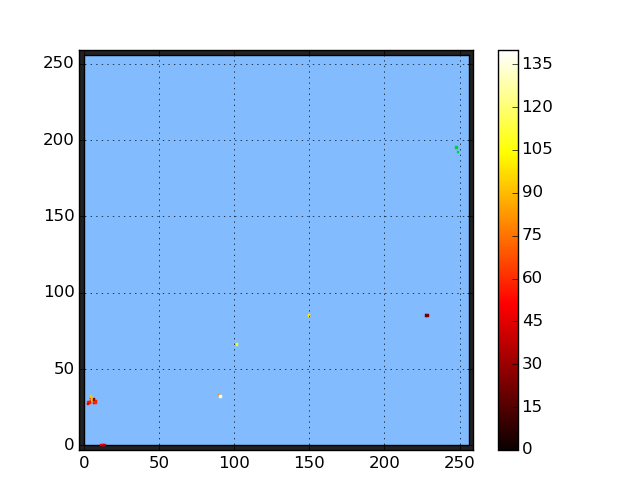
\includegraphics[width=0.7\textwidth]{assets/images/frame.png}
  \caption[The example output from the CERN@school job.]
  {\label{fig:localrunningframe}The example output from the CERN@school job.}
\end{figure}
%

For reference, that's a beta particle in the bottom left corner, and
five gammas in the rest of the frame! You can also find the source code
on the
\href{http://github.com/CERNatschool/particle-rate-plotter}{CERN@school
GitHub page}.


\clearpage

%%%%%%%%%%%%%%%%%%%%%%%%%%%%%%%%%%%%%%%%%%%%%%%%%%%%%%%%%%%%%%%%%%%%%%%%%%%%%%%
\section{Getting on the Grid}
\label{sec:onthegrid}
%%%%%%%%%%%%%%%%%%%%%%%%%%%%%%%%%%%%%%%%%%%%%%%%%%%%%%%%%%%%%%%%%%%%%%%%%%%%%%%
We have run local jobs so far. Now it's time to get on the grid - after
which, we will be able to configure Ganga to submit our jobs to the
GridPP DIRAC system and so access all of the computing and data
resources GridPP has to offer. The following sections will cover:

\begin{itemize}
\tightlist
\item
  Getting a grid certificate (Section~\ref{sec:gridcert});
\item
  Joining a Virtual Organisation (Section~\ref{sec:joinvo});
\item
  Logging on to GridPP DIRAC.
\end{itemize}

We'll find out more about what each of these steps mean and entail as we
go.

\begin{warningbox}{Thinking ahead}
\emph{Some of these steps require interaction with a human being. For example,
to get a grid certificate you have to visit your local Registration
Authority in person with photographic ID. Please bear this in mind
before you begin - it is not an automated process and may take a little
time. It will be worth it though!}
\end{warningbox}

Let's start by getting you a Grid certificate, shall we?

%=============================================================================
\subsection{Your Grid certificate}
\label{sec:gridcert}
%=============================================================================
Your grid certificate is your passport to the grid. It will give you
access to the vast array of computational resources that GridPP (and the
wLCG) has to offer. As such, getting a grid certificate is an
understandably non-trivial, multi-step process. For example, you will
need to identify yourself to your local Registration Authority (RA) so
that the grid knows who you are.

In concrete terms, a grid certificate is a .p12 file (i.e.~a pkcs12 web
browser certificate file) that you will later convert into a \emph{user
key} file and a \emph{user certificate} file. Encoded according to the
X.509 standard, these are used by the grid to confirm who are you are
and so give you access to grid resources.

%-----------------------------------------------------------------------------
\subsubsection{Requesting a Grid certificate}
\label{requesting-a-grid-certificate}
%-----------------------------------------------------------------------------
Grid certificates in the UK are managed by the
UK e-Science Certificate Authority\footnote{%
See \href{http://ngs.ac.uk/ukca}{http://ngs.ac.uk/ukca}}.
To start the process, you need to choose a web browser that you will have
consistent access to. We recommend Firefox as this process has been
tested and confirmed to work with Firefox on most Operating Systems.
This is because you need to use the same system for both requesting your
certificate and retrieving it when it is ready.

\begin{warningbox}{Temporary logins}
\emph{Do not use a temporary login anywhere when requesting a grid
certificate.}
\end{warningbox}

Using your browser of choice visit the CA portal\footnote{%
See \href{https://portal.ca.grid-support.ac.uk/caportal/}{https://portal.ca.grid-support.ac.uk/caportal/}}
and select the \emph{Request New User Certificate} option. This almost goes
without saying, but make sure you supply a \textbf{valid email address}
which you can access. You will also be asked to do things like supply a
PIN and passwords that you will need later on, so \textbf{make sure you
write everything down}!

\begin{infobox}{Registration Authroties}
\emph{You will need to select a Registration Authority (RA) as part of this
process. If your institution does not have its own RA, select the
nearest on the drop-down menu. You will need to visit the RA in person
with some photographic identification, so don't pick one that is too far
away! If no contact information is listed for a given RA, they will
almost certainly be retrievable using a Search Engine of Your Choice or
via their department's webpage. They will be delighted to hear from you!}
\end{infobox}

Further instructions will then be emailed to you at the email address
you have supplied during the registration process. Once that has
happened you should get a further email from someone at the RA asking
you to visit them in person to complete the validation process.

\begin{warningbox}{Who are you?}
\emph{You may also be asked to supply a letter of recommendation (or, rather,
an email from a suitable authority) explaining why you need to use the
grid and with whom you will be working. If you are unsure about who to
ask for this, please contact us\footnote{%
See \href{https://www.gridpp.ac.uk/contact}{https://www.gridpp.ac.uk/contact}}
and we should be able to help you out.}
\end{warningbox}

%-----------------------------------------------------------------------------
\subsubsection{Installing your Grid certificate in your web browser}
\label{installing-your-grid-certificate-in-your-web-browser}
%-----------------------------------------------------------------------------
Assuming all has gone to plan, you should receive a confirmation email
with a link that will let you download your grid certificate file and
install it in your browser. You will now be able to export and backup
your grid certificate using your browser's certificate management
functionality. This process will vary from browser to browser and from
OS to OS, so consult the
\href{http://www.ngs.ac.uk/ukca/certificates}{UK CA documentation} if in
doubt.

Congratulations - now you can be identified on the grid, you're ready to
join a \term{Virtual Organisation}.


%=============================================================================
\subsection{Joining a Virtual Organisation}
\label{sec:joinvo}
%=============================================================================
Your Grid certificate identifies you to the grid as an individual user,
but it's not enough on its own to allow you to use grid resources; you
also need to join a \term{Virtual Organisation} (VO). These are essentially
just user groups - typically one per experiment - and individual
Resource Centres (RCs) can choose to support work by users of a
particular VO. Most RCs support the four VOs associated with the Large
Hadron Collider (LHC) experiments. The sign-up procedure varies from VO
to VO. UK-based VOs typically require a manual approval step, while LHC
VOs require an active CERN account. If you are already part of an
experiment that is represented by a VO, they should provide you with any
specific instructions you need to join.

If you're interesting in using the grid but are not (yet) working as
part of a user community already represented by a VO, worry not. GridPP
have created a catch-all VO -
\href{https://voms.gridpp.ac.uk:8443/voms/gridpp/}{\texttt{gridpp}} -
and four Regional Virtual Organisations (RVOs) corresponding to the four
Tier 2s that can be joined to test out what the grid has to offer. Once
you have used these ``incubator'' VOs to see if the Grid meets your
needs, you can then think about creating your own Virtual Organisation
to represent your user community.

\begin{infobox}{Is there a VO for you already?}
\emph{Your user community may already have a VO associated with it. Check the
GridPP wiki page of supported VOs to see if you can join that to speed
things up.}
\end{infobox}

%-----------------------------------------------------------------------------
\subsubsection{Joining an incubator VO}
\label{joining-an-incubator-vo}
%-----------------------------------------------------------------------------
\begin{infobox}{Just browsing}
\emph{Some users have reported that the VOMS registration described below
fails using the Safari web browser. We have tried and tested the process
using Mozilla Firefox.}
\end{infobox}

\begin{infobox}{Trusting the VOMS servers}
\emph{Please ignore any ``untrusted connection'' warnings when accessing the
VOMS server pages. GridPP is aware that the VOMS server uses unsigned
certificates, but this situation is unlikely to be resolved any time
soon.}
\end{infobox}

%-----------------------------------------------------------------------------
\subsubsection{Joining the GridPP VO}
\label{joining-the-gridpp-vo}
%-----------------------------------------------------------------------------

To join the
\href{https://voms.gridpp.ac.uk:8443/voms/gridpp}{\texttt{gridpp}} VO,
visit
\href{https://voms.gridpp.ac.uk:8443/voms/gridpp/register/start.action}{this
page} using a browser that has your grid certificate installed and
follow the instructions.

%-----------------------------------------------------------------------------
\subsubsection{Joining a Regional VO}
\label{joining-a-regional-vo}
%-----------------------------------------------------------------------------
Likewise, you can join one of the four regional VOs:

\begin{itemize}
\item
\texttt{vo.londongrid.ac.uk}
\item
\texttt{vo.northgrid.ac.uk}
\item
\texttt{vo.scotgrid.ac.uk}
\item
\texttt{vo.southgrid.ac.uk}
\end{itemize}

\begin{infobox}{Confirming VO your membership}
\emph{Your VO membership request needs to be confirmed manually by one of the
VO administrators, so please wait for the membership confirmation email
to arrive before proceeding. You may wish to keep an eye on your junk
folder(s) too.}
\end{infobox}

Once you have joined a VO, congratulations - you are ready to start
using the Grid!


%=============================================================================
\subsection{Logging on with GridPP DIRAC}
\label{sec:logondirac}
%=============================================================================
There are many ways of accessing and using Grid resources. Larger
organisations - such as the four LHC experiments - have developed their
own frameworks, architectures and mechanisms to enable their members to
run jobs and access experimental data.

One such framework -- \term{DIRAC}~\cite{DIRAC2010} -- is used by
LHCb~\cite{LHCb2008}, but also many other Grid
projects, to manage grid jobs and storage.
You can read more about DIRAC
(Distributed Infrastructure with Remote Agent Control)
on their website\footnote{%
See \href{http://diracgrid.org}{http://diracgrid.org}}
or in~\cite{DIRAC2010},
but for our purposes all you need to
know for now is that DIRAC provides a way for you to access grid
resources without worrying too much about what's going on behind the
scenes.

%-----------------------------------------------------------------------------
\subsubsection{The GridPP DIRAC instance}
\label{the-gridpp-dirac-instance}
%-----------------------------------------------------------------------------
The Imperial College London GridPP Resource Centre (RC) hosts an
instance of DIRAC on behalf of GridPP~\cite{GRIDPPDIRAC2015a,GRIDPPDIRAC2015b}.
The GridPP DIRAC instance is is
capable of serving multiple VOs, providing grid job and data management
capabilities for smaller, non-LHC user communities wishing to make use
of GridPP resources. As a new user, you are automatically registered
with the GridPP DIRAC instance and the Virtual Organisations you have
joined. You can then test out various bits of grid functionality to
determine if grid computing will meet your needs and the needs of your
users.

You can interact with the Grid via the GridPP DIRAC web portal at:

\url{https://dirac.gridpp.ac.uk}

When you access the portal, you should
see yourself listed as a \textbf{Visitor} in drop-down menu in the
bottom-right corner of the browser. Once you have joined one or more
DIRAC-supported Virtual Organisations, you will be able to select which
VO you use DIRAC as using this drop-down menu.

\begin{infobox}{The GridPP DIRAC mailing list}
\emph{You should also join the GridPP DIRAC mailing list to keep informed of
the latest developments and receive notices of any downtime. You can
join the mailing list here.}
\end{infobox}

So you've accessed the GridPP DIRAC web portal. Congratulations!
However, as discussed, we'll be using GridPP DIRAC via the Ganga
interface. In order to do that, you'll need to install your Grid
certificate on your local machine - and the instructions for
doing this are in the next section.


%=============================================================================
\subsection{Preparing your Grid certificate}
\label{sec:certprep}
%=============================================================================
Ganga will assume that your grid certificate is in a certain location
and in a certain format in order to use it. Your grid certificate
therefore needs to be moved and prepared accordingly - which you can do
by following the instructions below.

%-----------------------------------------------------------------------------
\subsubsection{Moving your Grid certificate to your UI}
\label{moving-your-grid-certificate-to-your-ui}
%-----------------------------------------------------------------------------
The first thing to do is move your Grid certificate (the one you got
after following the instructions in Section~\ref{sec:gridcert})
%\href{../getting-on-the-grid/grid-certificate.md}{here}
to the \texttt{\textasciitilde{}/.globus/} directory in your home folder.

\begin{Shaded}
\begin{Highlighting}[]
\NormalTok{$ }\KeywordTok{cd} \NormalTok{~}
\NormalTok{$ }\KeywordTok{pwd}
\NormalTok{[}\KeywordTok{Your} \NormalTok{home directory.]}
\NormalTok{$ }\KeywordTok{mkdir} \NormalTok{.globus}
\NormalTok{$ }\KeywordTok{cp} \NormalTok{[The location of your certificate file.]/[Your certificate filename].p12 ./.globus/.}
\end{Highlighting}
\end{Shaded}

\begin{warningbox}{Certificates on CernVMs}
\emph{If you are using a CernVM and have moved your personal Grid certificate
file to it, you should change the password of the gridpp account so that
no-one else can use it. This can be done in the standard UNIX way with
the passwd command.}
\end{warningbox}

%-----------------------------------------------------------------------------
\subsubsection{Converting your Grid certificate}
\label{converting-your-grid-certificate}
%-----------------------------------------------------------------------------
In order to use your Grid certificate, you need to convert them into
separate certificate and key files. Don't worry, this straightforward
enough to do with the following commands:

\begin{Shaded}
\begin{Highlighting}[]
\NormalTok{$ }\KeywordTok{cd} \NormalTok{~/.globus}
\NormalTok{$ }\KeywordTok{openssl} \NormalTok{pkcs12 -in [Your certificate filename.].p12 -clcerts -nokeys -out usercert.pem}
\KeywordTok{Enter} \NormalTok{Import Password:}
\KeywordTok{MAC} \NormalTok{verified OK}
\NormalTok{$ }\KeywordTok{openssl} \NormalTok{pkcs12 -in [Your certificate filename.].p12 -nocerts -out userkey.pem}
\KeywordTok{Enter} \NormalTok{Import Password:}
\KeywordTok{MAC} \NormalTok{verified OK}
\KeywordTok{Enter} \NormalTok{PEM pass phrase:}
\KeywordTok{Verifying} \NormalTok{- Enter PEM pass phrase:}
\end{Highlighting}
\end{Shaded}

You will then need to change the file permission settings on the two
newly-generated files:

\begin{Shaded}
\begin{Highlighting}[]
\NormalTok{$ }\KeywordTok{chmod} \NormalTok{400 userkey.pem}
\NormalTok{$ }\KeywordTok{chmod} \NormalTok{600 usercert.pem}
\end{Highlighting}
\end{Shaded}

And that's it! You're now ready to use GridPP DIRAC with Ganga. It may
have seemed like a lot of work, but hopefully the next section
%\href{../example-workflow-grid/example-workflow-grid.md}{next section}
will demonstrate it will all have been worth it.


%=============================================================================
\subsection{Checklist}
\label{getting-on-the-grid---checklist}
%=============================================================================

\subsubsection{Your Grid certificate}\label{your-grid-certificate}

\begin{itemize}
\tightlist
\item
  I have requested a grid certificate from the
  \href{http://ngs.ac.uk/ukca}{UK Certificate Authority} (UKCA).
\item
  I know where my nearest
  \href{https://portal.ca.grid-support.ac.uk/caportal/pub/viewralist}{Registration
  Authority} (RA) is.
\item
  I have visited my nearest RA and confirmed my identity.
\item
  I have downloaded my grid certificate .p12 file and installed it in my
  browser.
\item
  I have backed up my grid certificate .p12 file in a secure location.
\end{itemize}

%-----------------------------------------------------------------------------
\subsubsection{Joining a Virtual Organisation -- Checklist}
\label{joining-a-virtual-organisation---checklist}
%-----------------------------------------------------------------------------

\begin{itemize}
\tightlist
\item
  I have submitted a request to join a Virtual Organisation (VO).
\item
  My request has been approved by a VO manager and I have received email
  confirmation of the approval.
\item
  I have followed all of the instructions in the confirmation email.
\end{itemize}

%-----------------------------------------------------------------------------
\subsubsection{First steps with GridPP DIRAC}
\label{first-steps-with-gridpp-dirac}
%-----------------------------------------------------------------------------

\begin{itemize}
\tightlist
\item
  I have accessed the \href{https://dirac.gridpp.ac.uk}{GridPP DIRAC web
  portal} with my Grid certificate-enabled browser.
\item
  I am recognised by the \href{https://dirac.gridpp.ac.uk}{GridPP DIRAC
  web portal} as a \emph{Visitor}.
\item
  I have joined the
  \href{https://mailman.ic.ac.uk/mailman/listinfo/gridpp-dirac-users}{GridPP
  DIRAC mailing list}.
\end{itemize}


%=============================================================================
\subsection{Testing}
\label{getting-on-the-grid---testing}
%=============================================================================

\subsubsection{Your Grid certificate}
\label{your-grid-certificate-testing}

\begin{itemize}
\tightlist
\item
  \textbf{Viewing your certificate details}: visit
  \href{https://portal.ca.grid-support.ac.uk/caportal/cert_owner}{this
  website} with the broswer in which your certificate is installed. You
  should see your grid certificate details displayed.
\end{itemize}

\subsubsection{Joining a Virtual Organisation}
\label{joining-a-virtual-organisation-testing}

\begin{itemize}
\tightlist
\item
  \textbf{Joining the GridPP VO}: Click
  \href{https://voms.gridpp.ac.uk:8443/voms/gridpp/user/search.action}{here}.
  If your request has been approved and confirmed, you should be listed
  as a VO member.
\item
  \textbf{Joining a Regional VO}: Click on
  \href{https://voms.gridpp.ac.uk:8443/voms/vo.londongrid.ac.uk/user/search.action}{\texttt{vo.londongrid.ac.uk}},
  \href{https://voms.gridpp.ac.uk:8443/voms/vo.northgrid.ac.uk/user/search.action}{\texttt{vo.northgrid.ac.uk}},
  \href{https://voms.gridpp.ac.uk:8443/voms/vo.scotgrid.ac.uk/user/search.action}{\texttt{vo.scotgrid.ac.uk}},
  or
  \href{https://voms.gridpp.ac.uk:8443/voms/vo.southgrid.ac.uk/user/search.action}{\texttt{vo.southgrid.ac.uk}}
  (depending on which VO you have attempted to join). If your request
  has been approved and confirmed, you should be listed as a VO member.
\end{itemize}

\subsubsection{First steps with DIRAC}
\label{first-steps-with-dirac-testing}

\begin{itemize}
\tightlist
\item
  \textbf{Accessing the GridPP DIRAC server}: access
  https://dirac.gridpp.ac.uk with your browser. If your grid certificate
  has been successfully installed in your browser, you should be asked
  to identify yourself with the certificate in question. You will then
  see the GridPP DIRAC server homepage. Check the bottom right-hand
  corner - if you can only see \emph{Visitor} and \textbf{not} your
  username and DN, something has gone wrong and you are not (or rather,
  your certificate is not) not registered with the GridPP DIRAC server.
\item
  \textbf{Joining the GridPP DIRAC mailing list}: once you have
  \emph{subscribed} and have \emph{been approved}, you should be able to
  view the
  \href{https://mailman.ic.ac.uk/mailman/roster/gridpp-dirac-users}{subscribers
  list} from the
  \href{https://mailman.ic.ac.uk/mailman/listinfo/gridpp-dirac-users}{list
  homepage} and confirm that you are indeed on it.
\end{itemize}


\clearpage

%%%%%%%%%%%%%%%%%%%%%%%%%%%%%%%%%%%%%%%%%%%%%%%%%%%%%%%%%%%%%%%%%%%%%%%%%%%%%%%
\section{Moving Your Workflow to the Grid}
\label{sec:gridrunning}
%%%%%%%%%%%%%%%%%%%%%%%%%%%%%%%%%%%%%%%%%%%%%%%%%%%%%%%%%%%%%%%%%%%%%%%%%%%%%%%
Now that you have your Grid certificate, and it is installed in your
browser and in your \texttt{\textasciitilde{}/.globus} directory, you're
ready to try submitting a job to the Grid with DIRAC.

%=============================================================================
\subsection{Activate DIRAC!}
\label{activate-dirac}
%=============================================================================
Thanks to CVMFS and the \href{https://github.com/ganga-devs/}{Ganga
team}, activating the GridPP DIRAC functionality is easy:

\begin{Shaded}
\begin{Highlighting}[]
\NormalTok{$ }\KeywordTok{source} \NormalTok{/cvmfs/ganga.cern.ch/dirac_ui/bashrc}
\end{Highlighting}
\end{Shaded}

You should now be able to tab-complete \texttt{dirac-} to see all of the
DIRAC commands that are available.

\begin{infobox}{DIRAC on CVMFS}
\emph{The inclusion of the pre-configured DIRAC UI in the Ganga CVMFS
repository means that you no longer need to install your own DIRAC UI.
Which makes life a lot easier}\ldots{}
\end{infobox}

%-----------------------------------------------------------------------------
\subsubsection{Generate a Grid proxy}
\label{generate-a-grid-proxy}
%-----------------------------------------------------------------------------
With DIRAC activated via CVMFS, you should now be able generate a
DIRAC-specific proxy to be used as a member of a DIRAC-enabled VO. Your
proxy is a file that identifies you on the Grid, letting the system know
that you're good for using its resources. If, for example, you were a
member of the \texttt{gridpp} catch-all VO you would use the following
commands to generate a proxy as a \texttt{gridpp\_user}:

\begin{Shaded}
\begin{Highlighting}[]
\NormalTok{$ }\KeywordTok{dirac-proxy-init} \NormalTok{-g gridpp_user -M}
\KeywordTok{Generating} \NormalTok{proxy... }
\KeywordTok{Enter} \NormalTok{Certificate password:}
\KeywordTok{Added} \NormalTok{VOMS attribute /gridpp }
\KeywordTok{Uploading} \NormalTok{proxy for gridpp_user... }
\KeywordTok{Proxy} \NormalTok{generated: }
\KeywordTok{subject}      \NormalTok{: /C=UK/O=eScience/OU=QueenMaryLondon/L=Computing/CN=ada lovelace/CN=proxy}
\KeywordTok{issuer}       \NormalTok{: /C=UK/O=eScience/OU=QueenMaryLondon/L=Computing/CN=ada lovelace}
\KeywordTok{identity}     \NormalTok{: /C=UK/O=eScience/OU=QueenMaryLondon/L=Computing/CN=ada lovelace}
\KeywordTok{timeleft}     \NormalTok{: 23:53:59}
\KeywordTok{DIRAC} \NormalTok{group  : gridpp_user}
\KeywordTok{path}         \NormalTok{: /tmp/x509up_u501}
\KeywordTok{username}     \NormalTok{: ada.lovelace}
\KeywordTok{properties}   \NormalTok{: NormalUser}
\KeywordTok{VOMS}         \NormalTok{: True}
\KeywordTok{VOMS} \NormalTok{fqan    : [}\StringTok{'/gridpp'}\NormalTok{] }
\end{Highlighting}
\end{Shaded}

If you get output that looks like the above, then it has all worked.

\begin{infobox}{Proxy status}
\emph{You can check the status of your DIRAC proxy at any time with the
dirac-proxy-info command.}
\end{infobox}

%-----------------------------------------------------------------------------
\subsubsection{Configuring Ganga to use the DIRAC backend}
\label{configuring-ganga-to-use-the-dirac-backend}
%-----------------------------------------------------------------------------
There's just one more step required before you can enjoy Grid running
with Ganga - you need to add the following to your
\texttt{\textasciitilde{}/.gangarc} configuration file:

\begin{Shaded}
\begin{Highlighting}[]
\NormalTok{[}\KeywordTok{Configuration}\NormalTok{]}
\KeywordTok{RUNTIME_PATH} \NormalTok{= GangaDirac}

\NormalTok{[}\KeywordTok{LCG}\NormalTok{]}
\KeywordTok{GLITE_SETUP} \NormalTok{= /cvmfs/ganga.cern.ch/dirac_ui/bashrc}

\NormalTok{[}\KeywordTok{DIRAC}\NormalTok{]}
\KeywordTok{DiracEnvSource} \NormalTok{= /cvmfs/ganga.cern.ch/dirac_ui/bashrc}

\NormalTok{[}\KeywordTok{defaults_DiracProxy}\NormalTok{]}
\KeywordTok{group} \NormalTok{= }\KeywordTok{<}\NormalTok{dirac user group}\KeywordTok{>}

\NormalTok{[}\KeywordTok{defaults_DiracFile}\NormalTok{]}
\KeywordTok{defaultSE} \NormalTok{= }\KeywordTok{<}\NormalTok{your SE of choice}\KeywordTok{>}
\end{Highlighting}
\end{Shaded}

where \texttt{\textless{}dirac\ user\ group\textgreater{}} should be
replaced by your default VO (e.g. \texttt{gridpp\_user}) and
\texttt{\textless{}your\ SE\ of\ choice\textgreater{}} should be
replaced by a suitable Storage Element, e.g.
\texttt{UKI-LT2-QMUL2-disk}.

\begin{infobox}{Finding an SE}
\emph{You can find a list of Storage Elements names by using the
dirac-dms-show-se-status command from the command line.}
\end{infobox}

You can then re-start Ganga; it will now be ready to connect to the
DIRAC backend.

%=============================================================================
\subsection{Run your job on the Grid}
\label{run-your-job-on-the-grid}
%=============================================================================
Now you're ready to run your job on the Grid. First, make a copy of the
\texttt{local\_job.py} script:

\begin{Shaded}
\begin{Highlighting}[]
\NormalTok{$ }\KeywordTok{cd} \OtherTok{$WORKINGDIR}
\NormalTok{$ }\KeywordTok{cp} \NormalTok{local_job.py dirac_job.py}
\NormalTok{$ }\KeywordTok{vim} \NormalTok{dirac_job.py}
\end{Highlighting}
\end{Shaded}

All you need to do is add the line \texttt{j.backend=Dirac()} before
submitting. That's it. That's all there is to it.

\begin{Shaded}
\begin{Highlighting}[]
\NormalTok{$ }\KeywordTok{cat} \NormalTok{dirac_job.py}
\KeywordTok{j} \NormalTok{= Job()}
\KeywordTok{j.name} \NormalTok{= }\StringTok{"CERN@school_dirac_01"}
\KeywordTok{j.application} \NormalTok{= Executable()}
\KeywordTok{j.application.exe} \NormalTok{= File(}\StringTok{'run.sh'}\NormalTok{)}
\KeywordTok{j.application.args} \NormalTok{= [}\StringTok{'B06-W0212/2014-04-02-150255/'}\NormalTok{]}
\KeywordTok{j.inputfiles} \NormalTok{= [ LocalFile(}\StringTok{'CERNatschool_backgroundrad_dataset.zip'}\NormalTok{) ]}
\KeywordTok{j.outputfiles} \NormalTok{= [ LocalFile(}\StringTok{'frames.json'}\NormalTok{), }\KeywordTok{LocalFile}\NormalTok{(}\StringTok{'log_process-frames.log'}\NormalTok{), }
\KeywordTok{LocalFile}\NormalTok{(}\StringTok{'output_images.tar'}\NormalTok{) ]}
\KeywordTok{j.backend} \NormalTok{= Dirac()}
\KeywordTok{j.submit}\NormalTok{()}
\end{Highlighting}
\end{Shaded}

(\emph{Oh, you may want to change the job name too}.)

If all has gone to plan, not only will you now be able to monitor your
job via your local Ganga instance (i.e.~with the \texttt{jobs} command),
you can see it on the \href{http://dirac.gridpp.ac.uk}{GridPP DIRAC web
portal}. Select \emph{Jobs} from the top-left menu below the URL bar,
then \emph{Job Monitor}.

\begin{warningbox}{Submission time}
\emph{Job submission to the Grid is not an instant process - a bit annoying
when you're submitting one or two test jobs (which is why local testing
wit Ganga is great!), but not such an issue with thousands of jobs. You
may wish to make a cup of tea, or do a bit of washing up.}
\end{warningbox}

Once the job shows up as green in the web portal, it's completed and you
can retrieve the output exactly as before.

So there you go - your first \emph{bona fida} grid job. Note that:

\begin{itemize}
\tightlist
\item Once your Grid stuff/DIRAC configuration was done, all it took to switch
to Grid running was a single line of code.
\item Thanks to CVMFS, you didn't have to do anything extra to deploy
your software to the Grid;
\item You didn't need to care about where the job actually ran - Ganga and DIRAC
sorted that all for you.
\end{itemize}

There's only one more thing to look at now before we've covered all of
the Grid-bases - getting data on and off the Grid. We'll look at that in
the next section.

\newpage

%=============================================================================
\subsection{Checklist}
\label{moving-the-example-workflow-to-the-grid---checklist}
%=============================================================================

\begin{itemize}
\tightlist
\item
  I can activate DIRAC by sourcing the DIRAC \texttt{bashrc} script from
  CVMFS;
\item
  I can generate a Grid proxy using the \texttt{dirac-proxy-init}
  command;
\item
  I can submit the CERN@school example workflow job to the Grid using
  Ganga;
\item
  I can monitor my Grid job(s) using the
  \href{https://dirac.gridpp.ac.uk}{GridPP DIRAC web portal}.
\end{itemize}


%=============================================================================
\subsection{Testing}
\label{moving-the-example-workflow-to-the-grid---testing}
%=============================================================================

\begin{itemize}
\item
  \textbf{Sourcing the DIRAC environment}: You can test the DIRAC
  environment variables have been set using the \texttt{echo} command.
  For example:

\begin{Shaded}
\begin{Highlighting}[]
\NormalTok{$ }\KeywordTok{echo} \OtherTok{$DIRAC}
\KeywordTok{/cvmfs/ganga.cern.ch/dirac_ui/}
\end{Highlighting}
\end{Shaded}

  If the DIRAC home directory on CVMFS is not listed, the environment
  variables have not been set correctly.
\item
  \textbf{Generating a DIRAC proxy}: You can test if your proxy
  generation has been successful by using the \texttt{dirac-proxy-info}
  command.
\item
  \textbf{Successful running of the CERN@school example job}: As with
  the locally-run example, once you have run and retrieved the images
  from the example job the first frame image should look something like
  that seen in Figure~\ref{fig:localrunningframe}.
\end{itemize}


\clearpage

%%%%%%%%%%%%%%%%%%%%%%%%%%%%%%%%%%%%%%%%%%%%%%%%%%%%%%%%%%%%%%%%%%%%%%%%%%%%%%%
\section{Putting Data on the Grid}
\label{sec:griddata}
%%%%%%%%%%%%%%%%%%%%%%%%%%%%%%%%%%%%%%%%%%%%%%%%%%%%%%%%%%%%%%%%%%%%%%%%%%%%%%%
We've now moved the local example workflow to the Grid.
However,
we've still only used data that's been present on our local system, and
we've manually retrieved the output to our local system. To harness the
full power of the Grid, we'll need to put data on it. We'll use tools
provided with DIRAC to do this, namely:

\begin{itemize}
\tightlist
\item The DIRAC File Catalog Command Line Interface (DFC CLI);
\item The DIRAC command line tools;
\item Some first steps with the DFC's metadata functionality.
\end{itemize}

First, though, let's look at some basic concepts in grid-based data
management.

%=============================================================================
\subsection{Storage Elements, File Catalogs, and Replicas}
\label{storage-elements-file-catalogs-and-replicas}
%=============================================================================
The first thing to wrap one's head around with distributed computing is
the notion that you don't really need to care about where your data is
stored. You may well be used to this concept if you've dealt with
cloud-based storage services such as Dropbox, Google Drive, or even
Amazon S3 storage. Your files are on one or more servers
\emph{somewhere}, and all that you need to know are the file names and
the directories that they're in to access them later.

It's the same with the grid. You upload your files to a grid
\textbf{Storage Element} (SE) and label them with a \textbf{Logical File
Name} (LFN) that gets registered in something called a \textbf{File
Catalog}. If you make copies of a particular file - a \textbf{replica} -
on one or more additional SEs, the locations of these replicas are
recorded in the File Catalog too.

\begin{infobox}{Storage Elements and replicas}
\emph{With most cloud-based storage services, you won't even really care about
the Storage Elements (or their non-grid equivalents, whatever the they
happen to be called) and file replicas. However, when considering
running grid jobs at a particular grid site, the location of your
replicas can matter (you'll want to make sure your data is available at
sites that will run jobs for your Virtual Organisation). We'll come back
to all of these concepts - and provide concrete examples - later.}
\end{infobox}

The GridPP DIRAC system provides a suite of tools to help you manage all
of this. If you're familiar with UNIX-based file systems you should find
it all pretty straightforward. We'll start with the
DIRAC File Catalog Command Line Interface.

%=============================================================================
\subsection{The DFC Command Line Interface}
\label{the-dfc-command-line-interface}
%=============================================================================
The DIRAC File Catalog (DFC) Command Line Interface (CLI), a.k.a. the
\textbf{DFC CLI}, provides a way of interacting with DIRAC's File
Catalog via - you guessed it - the command line. The DFC CLI lets you
manually upload and download files to Storage Elements (SEs), browse the
DFC associated with your Virtual Organisation (VO), create and remove
directories in the DFC, and manage the replicas associated with each
entry in the DFC.

\begin{infobox}{Using the DFC CLI}
\emph{The DFC CLI is great for small-scale tasks such as creating and tweaking
test data sets, but ultimately we will want to use scripts to help
coordinate large-scale upload operations and managing metadata
(i.e.~data about the data).}
\end{infobox}

%-----------------------------------------------------------------------------
\subsubsection{Getting started with the DFC CLI}
\label{getting-started-with-the-dfc-cli}
%-----------------------------------------------------------------------------

\term{Accessing the DFC CLI}

The DFC CLI is accessed via a DIRAC command, so we'll need to source our
DIRAC environment and generate a DIRAC proxy.

\begin{Shaded}
\begin{Highlighting}[]
\NormalTok{$ }\KeywordTok{source} \NormalTok{/cvmfs/ganga.cern.ch/dirac_ui/bashrc}
\NormalTok{$ }\KeywordTok{dirac-proxy-init} \NormalTok{-g gridpp_user -M}
\KeywordTok{Generating} \NormalTok{proxy... }
\KeywordTok{Enter} \NormalTok{Certificate password: }\CommentTok{# Enter your grid certificate password...}
\KeywordTok{.}
\KeywordTok{.} \NormalTok{[}\KeywordTok{Proxy} \NormalTok{information-based output.]}
\KeywordTok{.}
\end{Highlighting}
\end{Shaded}

\begin{warningbox}{Which VO?}
\emph{If you wish to use a different VO, replace gridpp with the name of the
VO in the commands in this section.}
\end{warningbox}

The DFC CLI is then started with the following DIRAC command:

\begin{Shaded}
\begin{Highlighting}[]
\NormalTok{$ }\KeywordTok{dirac-dms-filecatalog-cli} 
\KeywordTok{Starting} \NormalTok{FileCatalog client}

\KeywordTok{File} \NormalTok{Catalog Client }\OtherTok{$Revision}\NormalTok{: 1.17 }\OtherTok{$Date}\NormalTok{: }
            
\KeywordTok{FC}\NormalTok{:/}\KeywordTok{>}
\end{Highlighting}
\end{Shaded}

\begin{infobox}{DIRAC command groupings}
\emph{We'll come back to the DIRAC command line tools in the next section, but
the} \code{dirac-dms-} \emph{at the start of the command refers to the DIRAC Data
Management System tools. All DIRAC commands are grouped in this way
which, combined with tab completion, can be very handy for finding the
command you're looking for!}
\end{infobox}

The \texttt{FC:/\textgreater{}} at the command prompt tells you that
you're in the DFC CLI. You can now explore the DFC using commands that
are very similar to those used with a typical UNIX file system. Let's do
this now.

%-----------------------------------------------------------------------------
\subsubsection{Finding your user space in the DFC}
\label{finding-your-user-space-in-the-dfc}
%-----------------------------------------------------------------------------
Let's start by listing the root directories in the DFC, which will give
us a list of the Virtual Organisations supported by GridPP DIRAC:

\begin{Shaded}
\begin{Highlighting}[]
\KeywordTok{FC}\NormalTok{:/}\KeywordTok{>} \NormalTok{ls}
\KeywordTok{cernatschool.org}
\KeywordTok{gridpp}
\KeywordTok{vo.londongrid.ac.uk}
\KeywordTok{vo.northgrid.ac.uk}
\KeywordTok{vo.scotgrid.ac.uk}
\KeywordTok{vo.southgrid.ac.uk}
\end{Highlighting}
\end{Shaded}

We're using GridPP DIRAC as a member of \texttt{gridpp} VO, so let's
move into that directory.

\begin{Shaded}
\begin{Highlighting}[]
\KeywordTok{FC}\NormalTok{:/}\KeywordTok{>} \NormalTok{cd gridpp/user}
\end{Highlighting}
\end{Shaded}

If one hasn't been created for you already, you can create your own user
space on the VO's File Catalog like so:

\begin{Shaded}
\begin{Highlighting}[]
\KeywordTok{FC}\NormalTok{:/gridpp/user}\KeywordTok{>} \NormalTok{cd a}
\KeywordTok{FC}\NormalTok{:/gridpp/user/a}\KeywordTok{>} \NormalTok{mkdir ada.lovelace}
\KeywordTok{FC}\NormalTok{:/gridpp/user/a}\KeywordTok{>} \NormalTok{chmod 755 ada.lovelace}
\KeywordTok{FC}\NormalTok{:/gridpp/user/a}\KeywordTok{>} \NormalTok{ls -la}
\KeywordTok{drwxr-xr-x} \NormalTok{0 ada.lovelace gridpp_user 0 2015-12-16 10:24:54 ada.lovelace }
\KeywordTok{FC}\NormalTok{:/gridpp/user/a}\KeywordTok{>} \NormalTok{exit}
\end{Highlighting}
\end{Shaded}

\begin{infobox}{Your DIRAC username}
\emph{If you don't know your DIRAC username (which should be used as your user
directory), exit the DFC CLI and use the dirac-proxy-info command.}
\end{infobox}

\begin{infobox}{Listing files}
\emph{Using the} \code{-la} \emph{option with the}
\code{ls} \emph{command works just as it does with the
normal command line, allowing you to see file owners, groups (VOs),
permissions, etc.}
\end{infobox}

\begin{warningbox}{File permissions}
\emph{Don't forget to change the file permissions on your files so that other
users can't modify them.}
\end{warningbox}

You've now got your own space on the GridPP DFC. Let's put some files in
it.

%-----------------------------------------------------------------------------
\subsubsection{Uploading files}
\label{uploading-files}
%-----------------------------------------------------------------------------
Firstly, we'll need a file to upload. Any file will do, but to keep
things simple let's create one in a temporary directory:

\begin{Shaded}
\begin{Highlighting}[]
\NormalTok{$ }\KeywordTok{cd} \NormalTok{~}
\NormalTok{$ }\KeywordTok{mkdir} \NormalTok{tmp}\KeywordTok{;} \KeywordTok{cd} \NormalTok{tmp}
\NormalTok{$ }\KeywordTok{vim} \NormalTok{TEST.md }\CommentTok{# Or whichever editor you use...}
\NormalTok{$ }\KeywordTok{cat} \NormalTok{TEST.md}
\CommentTok{#Hello Grid!}
\KeywordTok{This} \NormalTok{is a test **MarkDown file**.}
\end{Highlighting}
\end{Shaded}

Next we'll need to know which \textbf{Storage Elements} are available to
us.

\begin{infobox}{Storage Elements}
\emph{Storage Elements} ``are physical sites where data are stored and
accessed, for example, physical file systems, disk caches or
hierarchical mass storage systems. Storage Elements manage storage and
enforce authorization policies on who is allowed to create, delete and
access physical files. They enforce local as well as Virtual
Organization policies for the use of storage resources. They guarantee
that physical names for data objects are valid and unique on the storage
device(s), and they provide data access. A storage element is an
interface for grid jobs and grid users to access underlying storage
through the Storage Resource Management protocol (SRM), the Globus Grid
FTP protocol, and possibly other interfaces as well.''

\emph{Credit: Open Science Grid (2012)}
\end{infobox}

We can list the available SEs with the following DIRAC command:

\begin{Shaded}
\begin{Highlighting}[]
\NormalTok{$ }\KeywordTok{dirac-dms-show-se-status} 
\KeywordTok{SE}                           \NormalTok{ReadAccess WriteAccess RemoveAccess CheckAccess }
\NormalTok{=============================================================================}
\NormalTok{[}\KeywordTok{...} \NormalTok{more disks ...]}
\KeywordTok{UKI-LT2-QMUL2-disk}           \NormalTok{Active     Active      Unknown      Unknown     }
\NormalTok{[}\KeywordTok{...} \NormalTok{more disks ...]}
\KeywordTok{UKI-NORTHGRID-LIV-HEP-disk}   \NormalTok{Active     Active      Unknown      Unknown}
\NormalTok{[}\KeywordTok{...} \NormalTok{more disks ...]}
\end{Highlighting}
\end{Shaded}

While we don't need to know the details of where and how our data will
be stored on an SE, we do need to know its name. We'll use the
\texttt{UKI-LT2-QMUL2-disk} SE for now. We add the file to the DFC as
follows using the \texttt{add} command, which takes the following
arguments:

\begin{verbatim}
add <LFN> <Local file name> <SE name>
\end{verbatim}

where:

\begin{itemize}
\tightlist
\item
  \texttt{\textless{}LFN\textgreater{}} is the \textbf{Logical File
  Name} (LFN) of the file in the DFC. This can either be relative to
  your current position in the DFC (which can be found with the
  \texttt{pwd} command in the DFC CLI), or made absolute by preceeding
  the name with a slash \texttt{/};
\item
  \texttt{\textless{}Local\ file\ name\textgreater{}} should be the name
  of the local file you want to upload. Again, this can be relative to
  wherever you were on your local system when you started the DFC CLI,
  or the absolute path to the file on your local system;
\item
  \texttt{\textless{}SE\ name\textgreater{}} is the name of the SE as
  retrived from the \texttt{dirac-dms-show-se-status} command.
\end{itemize}

Let's add our file to the grid now.

\begin{Shaded}
\begin{Highlighting}[]
\NormalTok{$ }\KeywordTok{dirac-dms-filecatalog-cli}
\KeywordTok{Starting} \NormalTok{FileCatalog client}

\KeywordTok{File} \NormalTok{Catalog Client }\OtherTok{$Revision}\NormalTok{: 1.17 }\OtherTok{$Date}\NormalTok{: }
            
\KeywordTok{FC}\NormalTok{:/}\KeywordTok{>} \NormalTok{cd /gridpp/user/a/ada.lovelace}
\KeywordTok{FC}\NormalTok{:/gridpp/user/a/ada.lovelace}\KeywordTok{>} \NormalTok{mkdir tmp}
\KeywordTok{FC}\NormalTok{:/gridpp/user/a/ada.lovelace}\KeywordTok{>} \NormalTok{cd tmp}
\KeywordTok{FC}\NormalTok{:/gridpp/user/a/ada.lovelace}\KeywordTok{>} \NormalTok{add TEST.md TEST.md UKI-LT2-QMUL2-disk}

\KeywordTok{File} \NormalTok{/gridpp/user/a/ada.lovelace/tmp/TEST.md successfully uploaded...}
\KeywordTok{FC}\NormalTok{:/gridpp/user/a/ada.lovelace/tmp}\KeywordTok{>}\NormalTok{ls -la}
\KeywordTok{-rwxrwxr-x} \NormalTok{1 ada.lovelace gridpp_user 47 2015-12-16 11:47:28 TEST.md}
\end{Highlighting}
\end{Shaded}

And there we go! Your first file has been uploaded to a Storage Element
on the grid. Have a biscuit. You've earned it.

%-----------------------------------------------------------------------------
\subsubsection{Replicating files}
\label{replicating-files}
%-----------------------------------------------------------------------------
Part of the joy of using the grid is being able to distribute
computational tasks to different sites. However, if you want to look at
the same data with a different task at different sites in an efficient
manner, ideally you'd need copies of that data at those sites. This
strategy also makes sense from a backup/redundancy perspective. We can
achieve this on the grid by using \emph{replicas}.

\begin{infobox}{Replicas}
\emph{A replica is a copy of a given file that is located on a different
Storage Element (SE). The file is identified by its Logical File Name
(LFN) in the DIRAC File Catalog (DFC). Associated with each LFN entry is
a list of SEs where replicas of the file can be found.}
\end{infobox}

To list the locations of replicas for a given file catalog entry, we use
the \texttt{replicas} command in the DFC CLI:

\begin{verbatim}
replicas <LFN>
\end{verbatim}

so continuing with our example:

\begin{Shaded}
\begin{Highlighting}[]
\KeywordTok{FC}\NormalTok{:/gridpp/user/a/ada.lovelace/tmp}\KeywordTok{>}\NormalTok{replicas TEST.md}
\KeywordTok{lfn}\NormalTok{: /gridpp/user/a/ada.lovelace/tmp/TEST.md}
\end{Highlighting}
\end{Shaded}

We replicate files with the \texttt{replicate} command:

\begin{verbatim}
replicate <LFN> <SE name>
\end{verbatim}

Let's replicate our test file to the Liverpool disk and check that the
replica list has been updated:

\begin{Shaded}
\begin{Highlighting}[]
\KeywordTok{FC}\NormalTok{:/gridpp/user/a/ada.lovelace/tmp}\KeywordTok{>}\NormalTok{replicate TEST.md UKI-NORTHGRID-LIV-HEP-disk}
\end{Highlighting}
\end{Shaded}

Replicas can be removed with the \texttt{rmreplica} command:

\begin{verbatim}
rmreplica <LFN> <SE name>
\end{verbatim}

Let's remove the Liverpool disk replica:

\begin{Shaded}
\begin{Highlighting}[]
\KeywordTok{FC}\NormalTok{:/gridpp/user/a/ada.lovelace/tmp}\KeywordTok{>}\NormalTok{rmreplica TEST.md UKI-NORTHGRID-LIV-HEP-disk}
\KeywordTok{lfn}\NormalTok{: /gridpp/user/a/ada.lovelace/tmp/TEST.md}
\KeywordTok{Replica} \NormalTok{at UKI-NORTHGRID-LIV-HEP-disk moved to Trash Bin}
\end{Highlighting}
\end{Shaded}

Finally, we can remove a file completely using the (somewhat familiar)
\texttt{rm} command:

\begin{verbatim}
rm <LFN>
\end{verbatim}

Let's tidy up our test file:

\begin{Shaded}
\begin{Highlighting}[]
\KeywordTok{FC}\NormalTok{:/gridpp/user/a/ada.lovelace/tmp}\KeywordTok{>}\NormalTok{rm TEST.md}
\KeywordTok{lfn}\NormalTok{: /gridpp/user/a/ada.lovelace/tmp/TEST.md}
\KeywordTok{File} \NormalTok{/gridpp/user/a/ada.lovelace/tmp/TEST.md removed from the catalog}
\end{Highlighting}
\end{Shaded}

%-----------------------------------------------------------------------------
\subsubsection{Downloading files}
\label{downloading-files}
%-----------------------------------------------------------------------------
Finally, we can download files using the DFC CLI with the \texttt{get}
command:

\begin{verbatim}
get <LFN> [<local directory>]
\end{verbatim}

Note that the local directory argument is optional. Let's download a
test file from the \texttt{gridpp} examples directory now:

\begin{Shaded}
\begin{Highlighting}[]
\KeywordTok{FC}\NormalTok{:/}\KeywordTok{>} \NormalTok{get /gridpp/userguide/WELCOME.md ./.}
\KeywordTok{FC}\NormalTok{:/}\KeywordTok{>} \NormalTok{exit}
\NormalTok{$ }\KeywordTok{cat} \NormalTok{WELCOME.md}
\CommentTok{#Welcome to GridPP!}

\KeywordTok{It} \NormalTok{looks like your download has worked. Congratulations!}
\NormalTok{$ }\KeywordTok{rm} \NormalTok{WELCOME.md}
\end{Highlighting}
\end{Shaded}

As we said earlier, the DFC CLI is only useful for small-scale
operations. On our way to scaling up, we can look at starting to
automate our workflows using scripts. In the next section we'll look at
how the DIRAC command line tools can help with this.


%=============================================================================
\subsection{The DIRAC Command Line Tools}
\label{the-dirac-command-line-tools}
%=============================================================================
So you've mastered the DFC Command Line Interface. Great stuff. What
you'll have probably noticed is that, while it's great for small-scale
operations, it's not ideal for doing things with lots of files on any
sort of scale. We will therefore want to take a look at the
\textbf{DIRAC command line tools} for data management.

\begin{infobox}{The command line tools}
\emph{All of the DIRAC command line tools start with}
\code{dirac-}. \emph{The data management tools start with}
\code{dirac-dms-}, \emph{as in Data Management System.
Press the tab key after typing} \texttt{dirac-dms-}
\emph{to see all of the available commands.}
\end{infobox}

Why are these commands useful? Well, it means you can use
\emph{scripting} to automate large-scale tasks involving many files.
There are many ways to \emph{script} the DIRAC (or indeed any command
line) commands. You've probably got your own preferred method that
reflects your coding background. For the purposes of the UserGuide,
we'll use simple bits of \textbf{Python} code (along with Python-based
file management libraries) to generate some simple \texttt{bash} scripts
that can then be run to perform the DIRAC operations we want to perform.

\begin{infobox}{Scripting DIRAC commands}
\emph{Of course, bash experts will be able to write scripts that perform all
of the operations below purely in bash. This is left as an exercise for
the reader - answers on a punch card please! (Also, we'll be using
Python for the DIRAC Python API, so it's not a bad thing to use Python
at this stage!)}
\end{infobox}

%-----------------------------------------------------------------------------
\subsubsection{Uploading files}
\label{uploading-files-tools}
%-----------------------------------------------------------------------------
The DIRAC file upload command takes the following form:

\begin{verbatim}
$ dirac-dms-add-file <LFN> <FILE> <SE>
\end{verbatim}

where:

\begin{itemize}
\tightlist
\item \texttt{\textless{}LFN\textgreater{}} is the Logical File Name
(LFN) of the entry for the file in the DIRAC File Catalog (DFC);
\item \texttt{\textless{}FILE\textgreater{}} is the path to the file on your
local machine, and;
\item \texttt{\textless{}SE\textgreater{}} is the name
of the destination Storage Element (SE).
\end{itemize}

\begin{infobox}{Finding SE names}
\emph{Remember, you can find the names of the available SEs with the
dirac-dms-show-se-status command.}
\end{infobox}

Suppose we have a number of files on our local machine in
\texttt{/home/gridpp/mydata/} that we want to upload to the grid. The
following Python code will generate a \texttt{bash} script that will
upload them to one of the Queen Mary Storage Elements:

\begin{Shaded}
\begin{Highlighting}[]
\NormalTok{$ cat make_upload_script.py}
\CommentTok{#!/usr/bin/env python}
\CommentTok{# -*- coding: utf-8 -*-}

\ImportTok{import} \NormalTok{os, glob}

\NormalTok{data_path }\OperatorTok{=} \StringTok{'/home/gridpp/mydata'}

\NormalTok{lfn_dir }\OperatorTok{=} \StringTok{'/gridpp/user/a/ada.lovelace/mydata/'}

\NormalTok{se }\OperatorTok{=} \StringTok{'UKI-LT2-QMUL2-disk'}

\NormalTok{s }\OperatorTok{=} \StringTok{"#!/bin/bash}\CharTok{\textbackslash{}n}\StringTok{"}

\ControlFlowTok{for} \NormalTok{my_file }\OperatorTok{in} \BuiltInTok{sorted}\NormalTok{(glob.glob(data_path }\OperatorTok{+} \StringTok{"/*"}\NormalTok{)):}
    \NormalTok{base_name  }\OperatorTok{=} \NormalTok{os.path.basename(my_file)}
    \NormalTok{upload_lfn }\OperatorTok{=} \NormalTok{os.path.join(lfn_dir, base_name)}
    \NormalTok{s }\OperatorTok{+=} \StringTok{"dirac-dms-add-file }\SpecialCharTok{%s}\StringTok{ }\SpecialCharTok{%s}\StringTok{ }\SpecialCharTok \NormalTok{(upload_lfn, my_file, se)}

\ControlFlowTok{with} \BuiltInTok{open}\NormalTok{(}\StringTok{"upload_script.sh"}\NormalTok{, }\StringTok{"w"}\NormalTok{) }\ImportTok{as} \NormalTok{sf:}
    \NormalTok{sf.write(s)}
\end{Highlighting}
\end{Shaded}

After you've generated a proxy and sourced the DIRAC environment, you
can run the generated script as follows:

\begin{Shaded}
\begin{Highlighting}[]
\NormalTok{$ }\KeywordTok{python} \NormalTok{make_upload_script.py}
\NormalTok{$ }\KeywordTok{chmod} \NormalTok{a+x upload_script.sh}
\NormalTok{$ }\KeywordTok{.} \KeywordTok{upload_script.sh}
\end{Highlighting}
\end{Shaded}

The results of this will, of course, depend on the contents of
\texttt{/home/gridpp/mydata/}, but all being well you should see the
message:

\begin{verbatim}
Successfully uploaded file to UKI-LT2-QMUL2-disk
\end{verbatim}

(or whichever SE you specified in your Python code) after each file has
been uploaded.

\begin{infobox}{Using Screen}
\emph{If you're uploading a lot of files, you may wish to consider using
something like the screen tool so that you can log off your terminal
session and come back to it later.}
\end{infobox}

And there we go! Multiple file uploads, all registered in the DIRAC File
Catalog, using a DIRAC command line tool and a bit of (admitedly
slightly clumsy) coding.

%-----------------------------------------------------------------------------
\subsubsection{Replicating files}
\label{replicating-files-tools}
%-----------------------------------------------------------------------------
Now, as we did with the DFC CLI, we can also make replicas of files,
list information about the replicas of a given file, and remove replicas
with the following command line tools:

\begin{verbatim}
dirac-dms-replicate-lfn <LFN> <SE>
dirac-dms-lfn-replicas <LFN>
dirac-dms-remove-replicas <LFN> <SE>
\end{verbatim}

Likewise, we can take the same approach with\ldots{}

%-----------------------------------------------------------------------------
\subsubsection{Downloading and removing files}
\label{downloading-and-removing-files-tools}
%-----------------------------------------------------------------------------

\begin{verbatim}
dirac-dms-get-file <LFN>
dirac-dms-remove-files <LFN>
\end{verbatim}

i.e.~the DIRAC command line tools exist for these operations. However,
getting information from the DFC about which files you would like to
replicate, download, remove, etc. is non-trivial when taking the command
line approach. This is especially true if you're writing scripts.

One approach is to use the \textbf{metadata} functionality the DIRAC
File Catalog provides to find files of interest.

\begin{infobox}{Metadata}
\term{Metadata} \emph{is data about the data. By assigning metadata to the files we
upload to the DIRAC File Catalog, we can perform queries that will
select only the files we are interested in. It also helps us to manage
our data. We'll find out more about the DFC's metadata functionality
later.}
\end{infobox}

The \texttt{dirac-dms-find-lfns} command finds LFNs based on the DFC
path and metadata query supplied as options. For example, to find all
files in the DFC that have been assigned to the experiment
\texttt{UserGuide}, we can type:

\begin{Shaded}
\begin{Highlighting}[]
\KeywordTok{dirac-dms-find-lfns} \NormalTok{Path=/ }\StringTok{"experiment=UserGuide"}
\NormalTok{\{}\StringTok{'experiment'}\NormalTok{: }\StringTok{'UserGuide'}\NormalTok{\}}
\KeywordTok{/gridpp/userguide/WELCOME.md}
\end{Highlighting}
\end{Shaded}

\texttt{experiment} here is the \textbf{metadata element} or
\textbf{index}. This is a string assigned to the file's LFN that, in
this case, has the value \texttt{UserGuide}. We can use the results of
this to download the files we want.

\begin{Shaded}
\begin{Highlighting}[]
\NormalTok{$ }\KeywordTok{dirac-dms-get-file} \NormalTok{/gridpp/userguide/WELCOME.md}
\NormalTok{\{}\StringTok{'Failed'}\NormalTok{: }\DataTypeTok{\{\}}\NormalTok{,}
 \StringTok{'Successful'}\NormalTok{: \{}\StringTok{'/gridpp/userguide/WELCOME.md'}\NormalTok{: }\StringTok{'/home/gridpp/tmp/WELCOME.md'}\NormalTok{\}\}}
\NormalTok{$ }\KeywordTok{cat} \NormalTok{WELCOME.md}
\CommentTok{#Welcome to GridPP!}

\KeywordTok{It} \NormalTok{looks like your download has worked. Congratulations!}
\end{Highlighting}
\end{Shaded}

Let's take a closer look at the DFC's metadata functionality using the
DFC CLI.


%=============================================================================
\subsection{First steps with the DIRAC metadata}
\label{first-steps-with-the-dirac-metadata-functionality}
%=============================================================================

%-----------------------------------------------------------------------------
\subsubsection{Finding files using metadata}
\label{finding-files-using-metadata}
%-----------------------------------------------------------------------------
When you're uploading vast amounts of data, it's nice to be able to find
it later. \textbf{Metadata} - data \emph{about the data} - can help with
this. DIRAC allows you to assign metadata such as strings, integers, and
floating point numbers to files and directories (via their Logical File
Names in the DIRAC File Catalog). You can then query the DFC to return a
list of the files you want.

For example, once you have sourced your DIRAC environment, generated a
proxy, and started the DFC CLI, you can find all files associated with
the \texttt{UserGuide} experiment like so:

\begin{Shaded}
\begin{Highlighting}[]
\KeywordTok{FC}\NormalTok{:/}\KeywordTok{>} \NormalTok{find / experiment=UserGuide}
\KeywordTok{Query}\NormalTok{: \{}\StringTok{'experiment'}\NormalTok{: }\StringTok{'UserGuide'}\NormalTok{\}}
\KeywordTok{/gridpp/userguide/WELCOME.md}
\KeywordTok{QueryTime} \NormalTok{0.98 sec}
\end{Highlighting}
\end{Shaded}

We have assigned the value \texttt{UserGuide} to the file
\texttt{WELCOME.md} for the \texttt{experiment} element or index. The
\texttt{find} command in the DFC CLI performs the query for us.

\begin{Shaded}
\begin{Highlighting}[]
\KeywordTok{FC}\NormalTok{:/}\KeywordTok{>} \NormalTok{help find}
 \KeywordTok{Find} \NormalTok{all files satisfying the given metadata information }
    
        \KeywordTok{usage}\NormalTok{: find [-q] [-D] }\KeywordTok{<}\NormalTok{path}\KeywordTok{>} \KeywordTok{<}\NormalTok{meta_name}\KeywordTok{>}\NormalTok{=}\KeywordTok{<}\NormalTok{meta_value}\KeywordTok{>} \NormalTok{[}\KeywordTok{<}\NormalTok{meta_name}\KeywordTok{>}\NormalTok{=}\KeywordTok{<}\NormalTok{meta_value}\KeywordTok{>}\NormalTok{]}
    
\KeywordTok{FC}\NormalTok{:/}\KeywordTok{>} \NormalTok{exit}
\end{Highlighting}
\end{Shaded}

In our query above, \texttt{\textless{}path\textgreater{}} was
\texttt{/} (i.e.~search the entire catalog from the base directory),
\texttt{\textless{}meta\_name\textgreater{}} was \texttt{experiment}
(i.e.~a metadata string index indicating to which experiment the data
belongs), and \texttt{\textless{}meta\_value\textgreater{}} was
\texttt{UserGuide} (OK, so the \texttt{UserGuide} isn't really an
experiment - at least not in the scientific sense - but you get the
idea!).

\begin{infobox}{Getting help with the DFC CLI}
\emph{You can get a list of all of the available commands in the DFC CLI by
using the help command. To list the instructions for a given command (as
above), type} \texttt{help {[}command{]}}.
\end{infobox}

There is only one file belonging to the \texttt{UserGuide} experiment in
the DFC, and it's a pretty harmless MarkDown file. But you can hopefully
see how, particularly when we start using multiple metadata indices with
different \emph{types}, DIRAC's metadata functionality is going to be
pretty useful.

%-----------------------------------------------------------------------------
\subsubsection{Assigning metadata to a file}
\label{assigning-metadata-to-a-file}
%-----------------------------------------------------------------------------
We can also use the DFC CLI to \emph{assign} metadata to our files.
Let's create a file with our favourite text editor and upload it to the
grid using the DFC CLI:

\begin{Shaded}
\begin{Highlighting}[]
\NormalTok{$ }\KeywordTok{vim} \NormalTok{TODO.md}
\NormalTok{$ }\KeywordTok{cat} \NormalTok{TODO.md}
\KeywordTok{ToDo}
\NormalTok{====}
\KeywordTok{*} \NormalTok{Email Charles re. engine}
\KeywordTok{*} \NormalTok{Re-do punchcards}
\KeywordTok{*} \NormalTok{Write to Dad}
\NormalTok{$ }\KeywordTok{dirac-dms-filecatalog-cli} 
\KeywordTok{Starting} \NormalTok{FileCatalog client}

\KeywordTok{File} \NormalTok{Catalog Client }\OtherTok{$Revision}\NormalTok{: 1.17 }\OtherTok{$Date}\NormalTok{: }
            
\KeywordTok{FC}\NormalTok{:/}\KeywordTok{>} \NormalTok{add /gridpp/user/a/ada.lovelace/TODO.md TODO.md UKI-LT2-QMUL2-disk}
\KeywordTok{File} \NormalTok{/gridpp/user/a/ada.lovelace/TODO.md successfully uploaded...}
\end{Highlighting}
\end{Shaded}

We can now set the \texttt{owner} index for the LFN using the
\texttt{meta\ set} command:

\begin{Shaded}
\begin{Highlighting}[]
\KeywordTok{FC}\NormalTok{:/}\KeywordTok{>} \NormalTok{meta set /gridpp/user/a/ada.lovelace/TODO.md owner ada.lovelace}
\KeywordTok{/gridpp/user/a/ada.lovelace/TODO.md} \NormalTok{owner ada.lovelace}
\end{Highlighting}
\end{Shaded}

We can now find the file again using the \texttt{find} command:

\begin{Shaded}
\begin{Highlighting}[]
\KeywordTok{FC}\NormalTok{:/}\KeywordTok{>} \NormalTok{find / owner=ada.lovelace}
\KeywordTok{Query}\NormalTok{: \{}\StringTok{'owner'}\NormalTok{: }\StringTok{'ada.lovelace'}\NormalTok{\}}
\KeywordTok{/gridpp/user/a/ada.lovelace/TODO.md}
\KeywordTok{QueryTime} \NormalTok{0.01 sec}
\end{Highlighting}
\end{Shaded}

As we've said before, the DFC CLI is useful for small-scale operations
on your data. Hopefully, though, you can start to appreciate the power
of \textbf{metadata} when it comes to organising your data and
performing analyses on it.

The most important thing for the moment, though, is that we can now put
data on the Grid (i.e.~on a Storage Element). This means we can use it
in our Grid jobs without needing to upload with our job as an
\texttt{inputfile}. We'll now complete making our example workflow fully
Grid-enabled in the next section.


%=============================================================================
\subsection{Checklist}
\label{putting-data-on-the-grid---checklist}
%=============================================================================

\begin{itemize}
\tightlist
\item
  I know what a Grid Storage Element (SE) is;
\item
  I know what the DIRAC File Catalog (DFC) is and what it is used for;
\item
  I know what LFN stands for and what it means with respect to the DFC;
\item
  I can access the DIRAC File Catalog Command Line Interface (DFC CLI);
\item
  I can find the Grid Storage Elements (SEs) available for me to use;
\item
  I can use tab-complete with \texttt{dirac-dms-} to find the available
  DIRAC command;
\item
  I can list the contents of my Virtual Organisations's area in the DFC
\item
  I can create a user area within this area and set the permissions
  accordingly;
\item
  Using both the DFC CLI and the DFC command line tools, I can:
\item
  upload and download files to and from an SE;
\item
  replicate files to another SE;
\item
  remove a replica from a specified SE;
\item
  remove a file from the DFC.
\item
  I know how to assign metadata to an LFN using the DFC CLI.
\end{itemize}


%=============================================================================
\subsection{Testing}
\label{putting-data-on-the-grid---testing}
%=============================================================================

\begin{itemize}
\tightlist
\item
  \textbf{Accessing data on a GridPP Storage Element (SE)}: If
  everything is setup correctly, the following commands should result in
  the output below:
\end{itemize}

\begin{Shaded}
\begin{Highlighting}[]
\NormalTok{$ }\KeywordTok{cd} \NormalTok{~}
\NormalTok{$ }\KeywordTok{mkdir} \NormalTok{tmp}
\NormalTok{$ }\KeywordTok{cd} \NormalTok{tmp}
\NormalTok{$ }\KeywordTok{dirac-dms-get-file} \NormalTok{LFN:/gridpp/userguide/WELCOME.md}
\NormalTok{\{}\StringTok{'Failed'}\NormalTok{: }\DataTypeTok{\{\}}\NormalTok{,}
 \StringTok{'Successful'}\NormalTok{: \{}\StringTok{'/gridpp/userguide/WELCOME.md'}\NormalTok{: }\StringTok{'/home/alovelace/tmp/WELCOME.md'}\NormalTok{\}\}}
\NormalTok{$ }\KeywordTok{cat} \NormalTok{WELCOME.md}
\CommentTok{#Welcome to GridPP!}

\KeywordTok{It} \NormalTok{looks like your download has worked. Congratulations! }
\end{Highlighting}
\end{Shaded}

\emph{You should have been able to follow everything else in the
previous subsections too, of course - but much of the input and output
will depend on your username, VO, etc. - the real test come when you
start putting data in your own user area in the next section!}



\clearpage

%%%%%%%%%%%%%%%%%%%%%%%%%%%%%%%%%%%%%%%%%%%%%%%%%%%%%%%%%%%%%%%%%%%%%%%%%%%%%%%
\section{Using Grid Data in Your Workflow}
\label{sec:griddatarunning}
%%%%%%%%%%%%%%%%%%%%%%%%%%%%%%%%%%%%%%%%%%%%%%%%%%%%%%%%%%%%%%%%%%%%%%%%%%%%%%%
The example workflow we've used so far isn't particularly sophisticated,
but it does allow us to demonstrate the final key concept we'll look at
here: incorporating Grid-based data in your workflows. Below we'll go
through:

\begin{itemize}
\tightlist
\item
  Putting the initial input data onto the Grid;
\item
  Using that data as the input to your workflow;
\item
  Writing the output data from your workflow to the Grid;
\item
  Retrieving the output from the Grid.
\end{itemize}

You'll need to have worked through Section~\ref{sec:gridrunning}
first -- mainly because we actually only need to tweak a few lines to
achieve what we want!

%=============================================================================
\subsection{Putting our input data onto the Grid}
\label{putting-our-input-data-onto-the-grid}
%=============================================================================
The first thing to do is put the ZIP file containing the raw frame data
into your user area on the DFC. You know how to do this (if not, have
another look at Section~\ref{sec:griddata})
so now we're getting into the realm of user areas, VOs, etc.
we're not going to give the explicit commands for this part. We'll also
leave you to come up with a LFN for the file, and choose which SE to use
(you might have a favourite by now).

\begin{itemize}
\tightlist
\item
  Download the ZIP file to your working directory;
\item
  Upload it to your user area in your VO's area in the DFC;
\item
  \textbf{Note down the LFN you assigned the file}. You'll need this
  below.
\end{itemize}

\begin{infobox}{Structuring your LFNs}
\emph{While the directories don't strictly exist with LFNs, it's useful to
keep things organised with sensible structuring/naming conventions. Use
the DFC CLI to create directories in your user area as required.}
\end{infobox}

%=============================================================================
\subsection{Getting data from the Grid}
\label{getting-data-from-the-grid}
%=============================================================================
Thanks to Ganga, there's actually not much to using a Grid-hosted data
file as input. All you need to do is add a \texttt{DiracFile} to the
job's \texttt{inputputfile} list with the LFN as the input argument. So
Ada's modified \texttt{dirac\_job.py} script would have the line:

\begin{Shaded}
\begin{Highlighting}[]
\KeywordTok{j.inputfiles} \NormalTok{= [ DiracFile(}\StringTok{'LFN:/.../CERNatschool_backgroundrad_dataset.zip'}\NormalTok{) ]}
\end{Highlighting}
\end{Shaded}

Replacing the \code{...} in the LFN with the full path.
The job will now retrieve the ZIP file from whichever Storage Element 1)
has a replica of the file and/or 2) is closest to the site running the
job to the working directory, just as it would with the
\texttt{LocalFile}.

\begin{infobox}{Replica loaction and management}
\emph{In fact, GridPP DIRAC will work out where is best to send your job based
upon where you have replicas of the file (i.e.~which SEs you
added/replicated it on). So once you're into optimisation territory,
replica management is something to think about.}
\end{infobox}

%=============================================================================
\subsection{Writing data to the Grid}
\label{writing-data-to-the-grid}
%=============================================================================
What about the output data? If you have an intermediary data layer
(i.e.~output that is used as input for another job/workflow) you may
wish to write the output to the Grid. This is possible with a few
tweaks, but there's a slight subtlety: GridPP DIRAC will assign LFNs for
your job output based on the DIRAC job ID and an LFN base specified in
your \texttt{.gangarc} file. This can be set with something like the
following:

\begin{Shaded}
\begin{Highlighting}[]
\NormalTok{[}\KeywordTok{DIRAC}\NormalTok{]}
\KeywordTok{DiracLFNBase} \NormalTok{= /gridpp/user/a/ada.lovelace}
\end{Highlighting}
\end{Shaded}

\begin{warningbox}{Preparing to submit}
\emph{Make sure you set this before starting Ganga and submitting your job(s).}
\end{warningbox}

Specifying which files get written to the Grid is then pretty similar to
specifying the input files - switch the \texttt{LocalFile} to
\texttt{DiracFile}:

\begin{Shaded}
\begin{Highlighting}[]
\KeywordTok{j.outputfiles} \NormalTok{= [ DiracFile(}\StringTok{'output_images.tar'}\NormalTok{) ]}
\end{Highlighting}
\end{Shaded}

With these changes made (and maybe a change of job name), you can now
submit your job.

%=============================================================================
\subsection{Retrieving the output from the Grid}
\label{retrieving-the-output-from-the-grid}
%=============================================================================
You already know how to
retrieve files from the Grid. The only extra detail you'll need to know
is the DIRAC job ID. \textbf{This is different to the job ID in Ganga}.
Both can be obtained with the following commands within Ganga:

\begin{Shaded}
\begin{Highlighting}[]
\KeywordTok{Ganga} \NormalTok{In [X]: j.id}
\KeywordTok{Ganga} \NormalTok{Out [X]: 1}

\KeywordTok{Ganga} \NormalTok{In [X]: j.backend.id}
\KeywordTok{Ganga} \NormalTok{Out [X]: 1234567}
\end{Highlighting}
\end{Shaded}

(i.e.~the DIRAC ID will have many more digits.)

The DIRAC ID will determine the LFN the output files are assigned. So
once the job has finished running, you should end up with something like
this:

\begin{Shaded}
\begin{Highlighting}[]
\NormalTok{$ }\KeywordTok{dirac-dms-filecatalog-cli} 
\KeywordTok{Starting} \NormalTok{FileCatalog client}

\KeywordTok{File} \NormalTok{Catalog Client }\OtherTok{$Revision}\NormalTok{: 1.17 }\OtherTok{$Date}\NormalTok{: }
            
\KeywordTok{FC}\NormalTok{:/}\KeywordTok{>} \NormalTok{cd gridpp/user/a/ada.lovelace/}
\KeywordTok{FC}\NormalTok{:/gridpp/user/a/ada.lovelace}\KeywordTok{>}\NormalTok{ls}
\KeywordTok{1234}
\KeywordTok{FC}\NormalTok{:/}\KeywordTok{>} \NormalTok{ls 1234}
\KeywordTok{1234567}
\KeywordTok{FC}\NormalTok{:/}\KeywordTok{>} \NormalTok{ls 1234/1234567}
\KeywordTok{frames.json}
\KeywordTok{output_images.tar}
\end{Highlighting}
\end{Shaded}

So the full LFN for the image archive is:

\begin{Shaded}
\begin{Highlighting}[]
\KeywordTok{LFN}\NormalTok{:/gridpp/user/a/ada.lovelace/1234/1234567/output_images.tar}
\end{Highlighting}
\end{Shaded}

This can be used to retrieve the file in the ways we have described
already - or used as an \texttt{inputfile} to another job.

So there we go - we've completely Grid-ified our example workflow. You
should now have all of the tools you need to start making your own
workflows Grid-ready. Of course, there's a lot more that can be done and
we'll mention some of the more advanced topics in the
next section.
But you should have plenty to get your teeth into for now!

%=============================================================================
\subsection{Checklist}
\label{using-grid-based-data-in-your-workflow---checklist}
%=============================================================================

\begin{itemize}
\tightlist
\item
  I can successfully modify the Grid workflow example to:
\item
  use an input \texttt{DiracFile} to with an lfn corresponding to data I
  have uploaded to the Grid;
\item
  write the output data to my user area on the DFC.
\item
  I can set the output LFN base in my Ganga configuration file;
\item
  I can run the modified Grid workflow example and retrieve the output
  from the Grid.
\end{itemize}


%=============================================================================
\subsection{Testing}
\label{using-grid-based-data-in-your-workflow---testing}
%=============================================================================

\begin{itemize}
\tightlist
\item
  \textbf{Successful running of the CERN@school example job}: Does
  Figure~\ref{fig:localrunningframe} look familiar? It really should do by now.
\end{itemize}


\clearpage

%%%%%%%%%%%%%%%%%%%%%%%%%%%%%%%%%%%%%%%%%%%%%%%%%%%%%%%%%%%%%%%%%%%%%%%%%%%%%%%
\section{What's Next?}
\label{sec:whatsnext}
%%%%%%%%%%%%%%%%%%%%%%%%%%%%%%%%%%%%%%%%%%%%%%%%%%%%%%%%%%%%%%%%%%%%%%%%%%%%%%%

%=============================================================================
\subsection{Uploading your software to CVMFS}
\label{uploading-your-software-to-cvmfs}
%=============================================================================
To start with, and if your software package/packages is/are small
enough, you can probably get away with uploading your software as
\texttt{LocalFile}s with your Grid job (perhaps using an archive file).
\emph{In fact, you may prefer this approach as http-based CVMFS repositories
are world-readable.}

However, at some point you and/or your Virtual Organisation are going to
want your own CVMFS repository. For small, UK-based VOs the best way to
do this is on the
\href{https://www.gridpp.ac.uk/wiki/RAL_Tier1_CVMFS}{RAL Tier-1
Stratum-0}. \href{mailto:info@gridpp.ac.uk}{Contact us} to find out more
about doing this - access to the repository is governed by your Grid
certificate.

In short, the process of uploading your software amounts to:

\begin{itemize}
\tightlist
\item \textbf{Generating a proxy with DIRAC}: as this will be used to
determine who you are and which repository you are accessing;
\item \textbf{Logging in to the repository}: You can then log in to your CVMFS
repository with:

\begin{Shaded}
\begin{Highlighting}[]
\NormalTok{$ }\KeywordTok{gsissh} \NormalTok{-p 1975 cvmfs-upload01.gridpp.rl.ac.uk}
\KeywordTok{Last} \NormalTok{login: [Date/time] from [hostname]}

   \KeywordTok{_.} \NormalTok{_.   o}\KeywordTok{|} \KeywordTok{_} \NormalTok{._}
  \KeywordTok{(_|(_||_|||(_)|} \KeywordTok{|}
       \KeywordTok{|}

          \KeywordTok{Location}\NormalTok{: r89.harwell.europe hpd r89rack137}
            \KeywordTok{Branch}\NormalTok{: cc34/cvmfs-uploader (sandbox}\KeywordTok{)}
         \KeywordTok{Archetype}\NormalTok{: ral-tier1}
       \KeywordTok{Personality}\NormalTok{: cvmfs-uploader}
  \KeywordTok{Operating} \NormalTok{System: sl640-x86_64}
     \KeywordTok{Snapshot} \NormalTok{Date: 2016-10-26}

\NormalTok{[}\DataTypeTok{\{vo-name\}}\KeywordTok{sgm@cvmfsXXXXX} \NormalTok{~]$ cd cvmfs_repo}
\KeywordTok{bin} \NormalTok{lib code README.md}
\end{Highlighting}
\end{Shaded}

\item
  \textbf{Retrieve your software}: You can now place your software in
  the repository, arranging it however works best for you. If your code
  is hosted in an online Git-based repository, simply
  \texttt{git\ clone} it straight to an appropriate directory.
\end{itemize}

\begin{infobox}{Looking at other CVMFS repositories}
\emph{You can take inspiration from other VOs. For example, you can browse the
ATLAS experiment's (CERN-hosted) CVFMS repository with:}
code{\$ ls /cvmfs/atlas.cern.ch/} \emph{and so on}.
\end{infobox}

\begin{warningbox}{Upload times}
Once put into the repository, it can be several hours before it becomes
available on the worker nodes - it's not instant. Make sure your
software is well-tested before putting it up - CVMFS is not appropriate
for software under development!
\end{warningbox}

However, once it \emph{is} on there, it's available everywhere. Which is
nice.

%=============================================================================
\subsection{Advanced DIRAC functionality}
\label{advanced-dirac-functionality}
%=============================================================================
DIRAC has a great deal of functionality of its own, particularly when
you start looking at the Python API. However, Ganga provides a nice
wrapper for much of this so you shouldn't need to touch it. You can find
out more on the \href{http://diracgrid.org/}{DIRAC homepage}, and check
out the source code on their \href{https://github.com/DIRACGrid}{GitHub
page}.

%=============================================================================
\subsection{Advanced Ganga functionality}
\label{advanced-ganga-functionality}
%=============================================================================
Likewise, there is a lot more to Ganga than we have covered here. Ganga
has its own documentation page:

\url{http://ganga.readthedocs.io}

which features things like:

\begin{itemize}
\tightlist
\item Configuration;
\item Job manipulation;
\item Splitters;
\item Post-processors;
\item Queues;
\item Etc.
\end{itemize}

The \href{https://github.com/ganga-devs/ganga}{GitHub repository} is
also worth watching for the latest updates and developments, as well as
raising any bugs or problems you may have in the
\href{https://github.com/ganga-devs/ganga/issues}{Issues} section.

\subsection{And finally\ldots{}}\label{and-finally}

Moving your workflow to the Grid won't necessarily be straightforward,
but at GridPP we're here to help -- if you've got a problem, just ask!
To keep up to date with the
UserGuide, watch the
\href{https://github.com/gridpp/user-guides}{\emph{UserGuide} GitHub
repository} to be notified of
\href{https://github.com/gridpp/user-guides/issues}{Issues} and Pull
Requests relating to additions or improvements to the \emph{UserGuide}.

Many thanks for reading so far, and happy Gridding!

\clearpage

%%%%%%%%%%%%%%%%%%%%%%%%%%%%%%%%%%%%%%%%%%%%%%%%%%%%%%%%%%%%%%%%%%%%%%%%%%%%%%%
\section{Troubleshooting}
\label{sec:troubleshooting}
%%%%%%%%%%%%%%%%%%%%%%%%%%%%%%%%%%%%%%%%%%%%%%%%%%%%%%%%%%%%%%%%%%%%%%%%%%%%%%%
This section contains brief notes on specific problems users have
encountered when working on specific systems, generally raised via the
\href{http://github.com/gridpp/user-guides/issues}{GitHub Issues page}.

\subsection{Ganga}\label{ganga}

\emph{Ganga isn't working.}

If you're having problems with Ganga, the best thing to do is to
\href{https://github.com/ganga-devs/ganga/issues}{raise an issue} with
the Ganga dev team through the
\href{https://github.com/ganga-devs/ganga/}{GitHub repository}. At the
time of writing, we've been using Ganga version 6.3.1 - but as Ganga is
under active development this may change so you may want to
\href{https://github.com/ganga-devs/ganga}{watch the repository too}.

\emph{Ganga throws errors relating to not being able lock files.}

If the file system your cluster is based on can't handle (or hasn't been
set up to allow) file locks, which Ganga uses. If your home directory is
on such a file system (e.g.~NFS), files in your
\texttt{\textasciitilde{}/gangadir} won't be lockable and Ganga won't
work. Assuming your cluster can't be reconfigured, the simplest thing to
do is change the location of your \texttt{gangadir} to somewhere that
can handle file locks, such as a scratch directory on the cluster. To do
this, set the \texttt{gangadir} option in
\texttt{\textasciitilde{}/.gangarc} to something like:

\begin{Shaded}
\begin{Highlighting}[]
\KeywordTok{gangadir} \NormalTok{= /scratch/alovelace/gangadir}
\end{Highlighting}
\end{Shaded}

and restart Ganga in the usual way.

\subsection{Miscellaneous problems}

\emph{My problem isn't listed here and search engines aren't helping
either.}

Raise an issue on the
\href{http://github.com/gridpp/user-guides/issues}{GitHub issues page}
and we'll see if we can help!

Good luck!

\clearpage

% Appendices

\begin{appendices}
%%%%%%%%%%%%%%%%%%%%%%%%%%%%%%%%%%%%%%%%%%%%%%%%%%%%%%%%%%%%%%%%%%%%%%%%%%%%%%%
\section{Creating a GridPP CernVM}
\label{sec:gridppcernvm}
%%%%%%%%%%%%%%%%%%%%%%%%%%%%%%%%%%%%%%%%%%%%%%%%%%%%%%%%%%%%%%%%%%%%%%%%%%%%%%%
If you don't have an account on a grid-ready cluster, don't worry - this
section will show you how to create a \textbf{Virtual Machine} (VM) that
will, essentially, act as a grid User Interface (UI) within whatever
operating system you happen to be using at the moment. We will do this
using the CernVM service~\cite{CernVM2015},
and create a guest CernVM on your host system.
There are a number of reasons to do this:

\begin{enumerate}
\def\labelenumi{\arabic{enumi}.}
\tightlist
\item
  The CernVM can act as a pre-built Grid User Interface (UI) that will
  give you all the tools you need (e.g.~a command line terminal, text
  editors, etc.) to get the most out of the Grid;
\item
  Your CernVM will also give you instant access to the CernVM-File
  System (CVMFS). A lot of the software we will use to manage our grid
  jobs and data is provided using this, with the huge bonus of \emph{not
  needing any installation by you}.
\item
  Most of the Grid tools we will use are compiled to run on Scientific
  Linux 6; With a CernVM you'll be able to use them out of the box;
\item
  The standard Grid Worker Nodes you'll be using to run your software on
  use SL6 machines. If your code runs on your CernVM, it will run on the
  Grid;
\item
  What's more, if everyone uses the CernVM as their Grid UI, we at
  GridPP will only have to support one operating system (i.e.~the SL6
  supplied with the CernVM). If we're singing from the same (virtual)
  hymn sheet, we'll be able to recreate your problems and help you solve
  them more easily.
\end{enumerate}

All you need to provide is the RAM and the hard disk space on your local
host machine.

\begin{infobox}{SL6 cluster access?}
\emph{If you already have access to a user account on an SL6 terminal, for
example on a university computing cluster, you can probably skip this
section.}
\end{infobox}

%=============================================================================
\subsection{An overview of the process}
\label{an-overview-of-the-process}
%=============================================================================
To create and configure a CernVM that will meet our needs, you will need
to:

\begin{enumerate}
\def\labelenumi{\arabic{enumi}.}
\tightlist
\item
  Install some virtualisation software on your host machine;
\item
  Download the appropriate CernVM Virtual Machine baseline image from
  the CernVM service;
\item
  Create a new guest CernVM using the CernVM image;
\item
  Configure the guest CernVM so that it has access to the host hard
  disk;
\item
  Configure the CernVM for Grid use by applying the GridPP
  \emph{contextualisation}.
\end{enumerate}

Let's look at each of these stages in a bit more detail.


%=============================================================================
\subsection{The virtualisation software}
\label{the-virtualisation-software}
%=============================================================================
You can find a list of compatible virtualisation software solutions on
the CernVM image download page
\href{http://cernvm.cern.ch/portal/downloads}{here}. It doesn't really
matter which you use but we've had success with
\href{http://download.virtualbox.org/virtualbox/4.3.12/VirtualBox-4.3.12-93733-Win.exe}{this
version of VirtualBox} (Windows 7).

\begin{warningbox}{Setting up the virtualisation software}
\emph{This is the one bit that's a bit tricky for us to support - how you do
this will depend on your local machine and its setup. Remember, search
engines and StackOverflow are your friends here.}
\end{warningbox}

%=============================================================================
\subsection{Creating your CernVM}
\label{creating-your-cernvm}
%=============================================================================
Depending on the virtualisation solution you picked (and got working)
above, download the baseline CernVM image file from here.

Then use your virtualisation software to create a new VM from the
downloaded image. You should be able to find instructions for how to do
this from your virtualisation software provider. Use as much RAM as you
can spare (up to about half of your host machine's total RAM) and use a
virtual hard disk of about 30 GB.

Once you have created your CernVM, but \emph{before you start it}, you
will need setup the \emph{contextualisation} for your CernVM.

\subsection{Contextualising your
CernVM}\label{contextualising-your-cernvm}

The CernVM service offers the ability to contextualise a CernVM with
pre-defined settings, environment variables, etc. that are put in place
when the CernVM is first booted. This is known as \emph{pairing} the VM.
You can create your own contextuallisations, but it is also possible for
individuals to create public contexts (e.g.~for LHC experiments, open
data initiatives, etc.) that anyone can use.

We have created such a context for GridPP. You can use it to get going
with the Grid. Importantly, you do not need a CERN account to do this,
so it is possible for anyone with a grid certificate to use it!

To pair your local CernVM with the GridPP context:

\begin{enumerate}
\def\labelenumi{\arabic{enumi}.}
\tightlist
\item
  \textbf{Log in to the CernVM service}: You can do this
  \href{https://cernvm-online.cern.ch/user/login}{here}. If you don't
  have a CERN account, you can register
  \href{https://cernvm-online.cern.ch/user/register}{here}.
\item
  \textbf{Visit the CernVM Marketplace}: This can be found
  \href{https://cernvm-online.cern.ch/market/list}{here}.
\item
  \textbf{Select the GridPP CernVM context}: Select \emph{Experimental}
  from the panel on the right, and then click on the
  \texttt{gridpp-cernvm} context.
\item
  \textbf{Boot up your local CernVM}: Once the boot process has
  finished, you should be presented with a login prompt. Don't enter
  anything yet.
\item
  \textbf{Pair with the GridPP context}: Returning to the GridPP CernVM
  Marketplace, click on the \emph{Pair} button on the panel on the
  right. This will generate a six-figure PIN.
\item
  \textbf{Apply the context to your VM}: Returning to your booted-up
  CernVM, enter the PIN (preceeded by a hash, as instructed at the login
  prompt). The CernVM webpage will now update indicating the VM has been
  successfully paired. Your VM will then be restarted and
  contextualised.
\item
  \textbf{Log in to your GridPP CernVM}: Once the context has been
  applied to your CernVM, you will be presented with a graphical login
  screen (as opposed to the text login prompt). Use the username
  \texttt{gridpp} and password \texttt{gridpp} to log in to your CernVM.
\end{enumerate}

And that's it! You now have a shiny new GridPP CernVM from which you'll
be able to access the Grid.

%=============================================================================
\subsection{Two final things}
\label{two-final-things}
%=============================================================================

\subsubsection{Configure git}\label{configure-git}

We'll be using \texttt{git} (and GitHub) to access various pieces of
code and scripts. The CernVM comes with \texttt{git} installed but
you'll need to configure it with your username and email address. This
can be done with the following commands:

\begin{Shaded}
\begin{Highlighting}[]
\NormalTok{$ }\KeywordTok{git} \NormalTok{config --global user.name }\StringTok{"Ada Lovelace"}
\NormalTok{$ }\KeywordTok{git} \NormalTok{config --global user.email alovelace@qmul.ac.uk}
\end{Highlighting}
\end{Shaded}

\subsubsection{Local hard disk access}\label{local-hard-disk-access}

Before we move on, it's important to note that you will need to be able
to access the hard disk of your host machine from that of your guest
CernVM. This is so that you can move any files that you need across to
the CernVM - most importantly, your Grid certificate file.

With VirtualBox, for example, this is achieved using the Shared Folders
functionality.

Before proceeding, you should make sure that you can access the parts of
your local hard disk that contain any software or data that you want to
copy across.

%=============================================================================
\subsection{Checklist}
\label{creating-a-grid-ui-with-a-gridpp-cernvm---checklist}
%=============================================================================

\begin{itemize}
\tightlist
\item
  I have installed some virtualisation software on my local machine that
  is compatible with the CernVM images listed at:

  \url{http://cernvm.cern.ch/portal/downloads}.
\item
  I have downloaded the corresponding CernVM image to my local machine
  from the CernVM image download page;
\item
  I have created a new guest VM on my local machine using the CernVM
  image;
\item
  I have registered with the CernVM service
  (or I am a CERN computing account holder);
\item
  I have generated a six-digit PIN to pair my CernVM with the GridPP
  context via the CernVM Marketplace;
\item
  I have entered the six-digit PIN (preceeded by the hash symbol) into
  the login prompt of my newly-booted CernVM;
\item
  I have logged in to my new GridPP CernVM using the \texttt{gridpp}
  user account;
\item
  I have accessed folders from my local machine's hard disk from my
  GridPP CernVM.
\end{itemize}


%=============================================================================
\subsection{Testing}
\label{creating-a-grid-ui-with-a-gridpp-cernvm---testing}
%=============================================================================

\begin{itemize}
\item
  \textbf{Downloading the CernVM image}: Your \texttt{Downloads} folder
  (or whichever location you chose to download the CernVM image file)
  contains the image file.

\begin{Shaded}
\begin{Highlighting}[]
\NormalTok{$ }\KeywordTok{cd} \NormalTok{~/Downloads}
\NormalTok{$ }\KeywordTok{ls} \NormalTok{-l }\KeywordTok{|} \KeywordTok{grep} \NormalTok{cernvm}
\KeywordTok{cernvm-3.5.1.iso}
\end{Highlighting}
\end{Shaded}
\item
  \textbf{Creating the CernVM}: When you start up your CernVM from your
  virtualisation software, you are eventually presented with a login
  screen.
\end{itemize}

\begin{Shaded}
\begin{Highlighting}[]
\KeywordTok{Welcome} \NormalTok{to CERN Virtual Machine, version 3.5.1.4}
  \KeywordTok{based} \NormalTok{on Scientific Linux release 6.6 (Carbon)}
  \KeywordTok{Kernel} \NormalTok{3.18.20-18.cernvm.x86_64 on an x86_64}

\KeywordTok{IP} \NormalTok{Address of this VM: [IP address]}
\KeywordTok{In} \NormalTok{order to apply cernvm-online context, use }\CommentTok{#<PIN> as user name.}

\KeywordTok{localhost} \NormalTok{login: _}
\end{Highlighting}
\end{Shaded}

\begin{itemize}
\item
  \textbf{Registering with the CernVM Service}: You can login via
  \href{https://cernvm-online.cern.ch/user/login}{this page}. When you
  access \href{https://cernvm-online.cern.ch/}{this page} you are
  redirected to the
  \href{https://cernvm-online.cern.ch/dashboard}{CernVM Dashboard}.
\item
  \textbf{Pairing your CernVM with the GridPP CernVM context}: After
  selecting the GridPP CernVM context in the
  \href{https://cernvm-online.cern.ch/market/list}{CernVM Marketplace}
  and clicking on the \emph{Pair} button on the right-hand panel, you
  are presented with a six-digit number. After entering the PIN into
  your CernVM's login screen (preceeded by the hash symbol), your CernVM
  reboots to display a graphical CernVM login screen. Meanwhile, the
  CernVM Pairing web page has updated to display the message,
  \textgreater{} \textbf{Setup instance - Completed} \textgreater{}
  \textgreater{} Your vm is now paired with CernVM Online! Upon logging
  in to your new CernVM with the username \texttt{gridpp} and the
  password \texttt{gridpp}, you are presented with the CernVM desktop.
\item
  \textbf{Accessing your local machine's hard disk from you CernVM}: You
  can access (from the command line or otherwise) folders on your local
  machine's hard disk on the GridPP CernVM. So (for example) if you're
  using VirtualBox with the \emph{Shared Folders} functionality, after
  adding the folders you want access to via the VM's \emph{Settings} and
  rebooting the VM you'll do something like this:

\begin{Shaded}
\begin{Highlighting}[]
\NormalTok{$ }\KeywordTok{sudo} \NormalTok{usermod -a -G vboxsf gridpp}
\NormalTok{[}\KeywordTok{sudo}\NormalTok{] password for gridpp: }\CommentTok{# Enter 'gridpp' here.}
\end{Highlighting}
\end{Shaded}

  before loggin out and logging in again. You'll then be able to access
  the folders you specified.

\begin{Shaded}
\begin{Highlighting}[]
\NormalTok{$ }\KeywordTok{cd} \NormalTok{/media/sf_alovelace/ }\CommentTok{# Shared Folder "alovelace" }
\NormalTok{$ }\KeywordTok{ls}
\KeywordTok{punch-card-01.dat} \NormalTok{dad-poem-001.txt my-poem-005.txt}
\end{Highlighting}
\end{Shaded}
\end{itemize}


\end{appendices}

\clearpage

%
%%%%%%%%%%%%%%%%%%%%%%%%%%%%%%%%%%%%%%%%%%%%%%%%%%%%%%%%%%%%%%%%%%%%%%%%%%%%%%%
% Bibliography
%%%%%%%%%%%%%%%%%%%%%%%%%%%%%%%%%%%%%%%%%%%%%%%%%%%%%%%%%%%%%%%%%%%%%%%%%%%%%%%
%
\section*{References}
\bibliographystyle{unsrt.bst}
\bibliography{GridPP}
%
%------------------------------------------------------------------------------

\newpage

%%%%%%%%%%%%%%%%%%%%%%%%%%%%%%%%%%%%%%%%%%%%%%%%%%%%%%%%%%%%%%%%%%%%%%%%%%%%%%%
\section*{Acknowledgements}
\label{sec:ack}
%%%%%%%%%%%%%%%%%%%%%%%%%%%%%%%%%%%%%%%%%%%%%%%%%%%%%%%%%%%%%%%%%%%%%%%%%%%%%%%
The author would like to thank GridPP Collaboration members Steve Jones
(Liverpool) and Steve Lloyd (QMUL), as well as the students from the
\href{http://researchinschools.org}{Institute for Research in Schools},
for providing invaluable feedback on the initial drafts of the
\emph{GridPP UserGuide}.
Andrew McNab (Uni. Manchester) has provided invaluable technical support
for the operation and maintenance of the
\href{http://www.gridpp.ac.uk}{GridPP website} on which the online
version of this guide is hosted\footnote{%
See \href{http://www.gridpp.ac.uk/userguide}{http://www.gridpp.ac.uk/userguide}}.
%
Much inspiration for the structure and
philosophy of the \emph{GridPP UserGuide} has been drawn from Michael
Hartl's \emph{\href{https://ww.railstutorial.org}{Ruby on Rails
Tutorial}} - an excellent read (even if you're not particularly fussed
about Ruby on Rails). We are also grateful to
\href{http://github.com}{GitHub} for our
\href{http://github.com/gridpp}{Organizational Repository} -- thanks!

This work was supported by the UK Science and Technology Facilities Council
(STFC) via the GridPP Collaboration~\cite{gridpp2006,gridpp2009}
and grant ST/N00101X/1 as part of work with the CERN@school research
programme.

%%%%%%%%%%%%%%%%%%%%%%%%%%%%%%%%%%%%%%%%%%%%%%%%%%%%%%%%%%%%%%%%%%%%%%%%%%%%%%%
\section*{About the author}
\label{sec:author}
%%%%%%%%%%%%%%%%%%%%%%%%%%%%%%%%%%%%%%%%%%%%%%%%%%%%%%%%%%%%%%%%%%%%%%%%%%%%%%%
Tom Whyntie is Public Engagement Fellow at the
\href{http://ph.qmul.ac.uk}{School of Physics \& Astronomy},
\href{http://www.qmul.ac.uk}{Queen Mary University of London}. He is
supported by the UK's \href{http://www.stfc.ac.uk}{Science and
Technology Facility Council} (STFC) through their
\href{http://www.stfc.ac.uk/funding/fellowships/public-engagement-fellowships/public-engagement-fellows/}{Public
Engagement Fellowship} programme and through the
\href{https://www.gridpp.ac.uk}{GridPP Project}. Having used the
Worldwide LHC Computing Grid (WLCG) extensively during his time on the
\href{http://cms.web.cern.ch/}{Compact Muon Solenoid} (CMS) experiment
at \href{http://cern.ch}{CERN}'s Large Hadron Collider, Tom works as
part of the GridPP Community to engage as many people as possible with
the Grid through GridPP's New User Engagement Programme. He is also
consultant scientist for the
\href{http://researchinschools.org}{CERN@school programme},
Scientific Officer for the \href{http://researchinschools.org}{Institute
for Research in Schools}, and Software Coordinator for the
\href{http://moedal.web.cern.ch}{MoEDAL Collaboration}.

\newpage


%%%%%%%%%%%%%%%%%%%%%%%%%%%%%%%%%%%%%%%%%%%%%%%%%%%%%%%%%%%%%%%%%%%%%%%%%%%%%%%
\section*{Version History}
%%%%%%%%%%%%%%%%%%%%%%%%%%%%%%%%%%%%%%%%%%%%%%%%%%%%%%%%%%%%%%%%%%%%%%%%%%%%%%%
%______________________________________________________________________________
\begin{table}[h]
\caption{\label{tab:version}Version history.}
\lineup
\begin{indented}
\item[]\begin{tabular}{@{}cllc}
\br
\centre{1}{$\quad$Version    $\quad$} & 
\centre{1}{$\quad$Description$\quad$} &
\centre{1}{$\quad$DOI        $\quad$} &
\centre{1}{$\quad$Author     $\quad$} \\
\mr
1.0 & Initial version. & \href{http://dx.doi.org/10.5281/zenodo.222702}{10.5281/zenodo.222702} & TW \\
\br
\end{tabular}
\end{indented}
\end{table}
%______________________________________________________________________________

\end{document}
